% 独自のコマンド

% ■ アブストラクト
%  \begin{jabstract} 〜 \end{jabstract}  :日本語のアブストラクト
%  \begin{eabstract} 〜 \end{eabstract}  :英語のアブストラクト

% ■ 謝辞
%  \begin{acknowledgment} 〜 \end{acknowledgment}

% ■ 文献リスト
%  \begin{bib}[100] 〜 \end{bib}


\newif\ifjapanese

\japanesetrue  % 論文全体を日本語で書く(英語で書くならコメントアウト)

\ifjapanese
  % \documentclass[a4j,twoside,openright,11pt]{jreport} % 両面印刷の場合。余白を綴じ側に作って右起こし。 >>bindermode<<
  \documentclass[a4j,11pt]{jreport}                  % 片面印刷の場合。 >>nobindermode<<
  \renewcommand{\bibname}{参考文献}
  \newcommand{\acknowledgmentname}{謝辞}
\else
  \documentclass[a4paper,11pt]{report}
  \newcommand{\acknowledgmentname}{Acknowledgment}
\fi
\usepackage{sty/thesis}
\usepackage{ascmac}
\usepackage{graphicx}
\usepackage{multirow}
\usepackage{url}
\usepackage[dvipdfmx]{hyperref}
\bibliographystyle{jplain}

% \bindermode  % バインダー用余白設定 >>bindermode<<

% 日本語情報(必要なら)
\jclass  {卒業論文}                             % 論文種別
\jtitle    {ネットワークを活用した\\高解像度映像伝送システムの設計と実装}    % タイトル。改行する場合は\\を入れる
\juniv    {慶應義塾大学}                  % 大学名
\jfaculty  {環境情報学部}               % 学部、学科
\jauthor  {山中 勇成}                       % 著者
\jhyear  {28}                                   % 平成○年度
\jsyear  {2016}                                 % 西暦○年度
\jkeyword  {4K, IP伝送, 映像配信システム, FPGA}     % 論文のキーワード
\jproject{徳田・村井・楠本・中村・高汐・バンミーター・植原・三次・中澤・武田 合同研究プロジェクト} %プロジェクト名
\jdate{2017年1月}

% 英語情報(必要なら)
\eclass  {Bachelor's Thesis}                            % 論文種別
\etitle    {Design and Implementation of Delivery System for High Resolution Video Utilizing Network}      % タイトル。改行する場合は\\を入れる
\euniv  {Keio University}                             % 大学名
\efaculty  {Bachelor of Arts in Environmental Information}  % 学部、学科
\eauthor  {Yusei Yamanaka}                           % 著者
\eyear  {2016}                                        % 西暦○年度
\ekeyword  {4K, Over IP, Video Streaming, FPGA}          % 論文のキーワード
\eproject{Tokuda/Murai/Kusumoto/Nakamura/Takashio/Van Meter/Uehara/Mitsugi/Nakazawa/Takeda Labs}                 %プロジェクト名
\edate{January 2017}

\begin{document}

\ifjapanese
  \jmaketitle    % 表紙(日本語)
\else
  \emaketitle    % 表紙(英語)
\fi

% ■ アブストラクトの出力 ■
%	◆書式:
%		begin{jabstract}〜end{jabstract}	:日本語のアブストラクト
%		begin{eabstract}〜end{eabstract}	:英語のアブストラクト
%		※ 不要ならばコマンドごと消せば出力されない。

% 日本語のアブストラクト
\begin{jabstract}

現行のハイビジョン放送を超える画質である、4K・8K映像の普及が世界中で加速している。
4K映像の帯域は2K映像と比較すると約4倍、現行のハイビジョン放送と比較すると約8倍になる。
既存の同軸ケーブルで4K映像を伝送するには、より太く短いケーブルを使用するか、既存のケーブルを複数本の束にして使用する必要があり、現場での扱いやすさに課題がある。
% また、4K映像に対応するためには、移行期間も含めHDと4Kに対応した映像機器のリプレースにコストがかかったりなど課題もある。
そのため、映像制作現場では、映像機器と比べて比較的安価なネットワーク機器と光ファイバーを使った伝送をする、Video over IP化が進んでいる。
光ファイバーにすることによる現場でのケーブル扱いやすさの向上が見込め、IP化をすることによる映像のリターンや制御情報、付加情報の伝送が可能になる。

本研究では、まず映像制作現場の構成を調べ、IP伝送装置の要件を調査した。
要件の1つである遅延の許容値を調査するため、映像用のスイッチャーをブラウザ上で再現し、遅延を加えて描画する実験環境を構築した。
これを用いて、映像遅延許容値の実験を行ったところ、133.33msの映像遅延まで「遅延を許容できる」と回答した被験者が全体の9割であった。
% したがって、IP伝送装置の要件として映像遅延は133.33ms以内が望ましいことがわかった。

本研究では、この要件を満たすIP伝送装置としてソフトウェアとハードウェアによる伝送装置の設計、実装を行った。
ソフトウェア実装では、4K映像キャプチャーボードと10Gbpsのネットワークカードを有する汎用マシン上でIP伝送を行うソフトウェアを実装した。
また、ハードウェア実装では、Xilinxの7-Series FPGAボードを用いてIP伝送装置を実装した。

実装したソフトウェアとハードウェアについて、理想的なトラフィックを送信しているか、133.33ms以内の遅延を達成しているか、などを計測した。
トラフィックを計測した結果、ハードウェア実装では理想的なデータを送信していたが、ソフトウェア実装では処理の問題により理想的なデータを送信できていなかった。
遅延を計測した結果、ソフトウェアとハードウェアではそれぞれ199.99ms、33ms以内の遅延があることがわかった。
この結果から、ソフトウェア実装では映像制作現場において必要な要件を満たせないが、ハードウェア実装ではその要件を満たすことができ、映像制作現場で十分に活用できることがわかった。

% 本研究では、実装を行うために必要となる、映像制作現場におけるIP伝送装置の要件を調査した。調査では映像の遅延が133.33msまでであれば「遅延を許容できる」と回答した人が9割であった。
% 汎用的なビデオインターフェースであるHDMIから、映像をIPパケット化し、非圧縮の4K映像を伝送するシステムを設計、実装する。

% 本研究では、4K映像キャプチャーボード、10Gbpsネットワークインターフェースカードを備えた汎用的なコンピューターで実装したソフトウェアと、Xilinxの7-Series FPGAボードで実装したハードウェアの両方を実装した。

% 評価として、実装したソフトウェア、実装したハードウェアのそれぞれにおいてトラフィック、遅延を計測した。
% ソフトウェアではおよそ199.99msの遅延があるが、ハードウェアでは33ms以内の遅延となった。
% 結果として、映像制作現場における要件を満たすことがでソフトウェア実装では困難であり、FPGAによるハードウェア実装が優位であることがわかった。

\end{jabstract}


% 英語のアブストラクト
\begin{eabstract}

In recent years, the spread of 4K / 8K images is accelerating all over the world.
The bandwidth of 4K video is about 4 times as compared with 2K video, and it is about 8 times as compared with the current high vision broadcasting, and the transmission method and its cost are the issues.
For this reason, in the video industry, Video over IP is advancing, utilizing relatively inexpensive network resources compared to video equipment, to transmit.

In this research, we first examined the composition of video production site and investigated the requirements of IP transmission equipment.
In order to investigate the tolerance of delay which is one of the requirements, we constructed an experimental environment in which a switcher for video is reproduced on the browser, and drawing is performed with delay added.
Using this, we conducted a physical exercise experiment of video delay. As a result, 90% of the subjects responded that "delay can be tolerated" until the video delay of 133.33 ms.
Therefore, we found that the video delay is desirable to be within 133.33 ms as a requirement of the IP transmission device.

In this research, we designed and implemented a transmission device by software and hardware as an IP transmission device satisfying this requirement.
In software implementation, we implemented software that performs IP transmission on a general purpose machine with 4K video capture board and 10 Gbps network card.
In the hardware implementation, an IP transmission device was implemented using Xilinx's 7-Series FPGA board.

We measured whether the ideal traffic is being transmitted or delayed within 133.33 ms for the implemented software and hardware.
As a result of measuring traffic, ideal data was transmitted by hardware implementation, but software implementation was not able to transmit ideal data due to processing problems.
Also, as a result of delay measurement, it was found that software and hardware had delays of within 199.99 ms and 33 ms respectively.
From the results, it was found that at the video production site, software implementation experienced delays, but hardware implementations will not be delayed and can be fully utilized at the video production site.

\end{eabstract}
  % アブストラクト。要独自コマンド、include先参照のこと

\tableofcontents  % 目次
\listoffigures    % 表目次
\listoftables     % 図目次

\pagenumbering{arabic}

\chapter{序論}
\label{chap:introduction}

\section{本論文の背景}
近年、現行のハイビジョン放送を超える高解像度な画質による、4K・8K映像の普及が世界中で加速している。また、日本でも東京2020オリンピック・パラリンピックに向け、総務省が4K・8K映像の普及を後押しをしている。

現在の放送業界では、同軸ケーブルを使用するSDIと呼ばれる伝送規格で映像を伝送する事が一般的である。また、ハイビジョン放送の制作では、1080iと呼ばれる有効走査線数1080本のインターレース方式が一般的である。
現行のハイビジョンと比較すると、4K映像の帯域は約8倍にもなり、伝送方法とそのコストが課題となっている。

SDIでは4K映像の伝送を目的として、SMPTE ST-2081\cite{smpte-st-2081}、および、SMPTE ST-2082\cite{smpte-st-2082}により、6G-SDIと12G-SDIが定められている。
しかし、現行のハイビジョンで使用されるHD-SDIと比較すると、高周波による減衰を少なくするために、より太く短い同軸ケーブルを使用しなければならず、現場での扱いづらさが課題である。

多くの放送局のスタジオなどで使用しているカメラでは、カメラ本体とCCU(カメラコントロールユニット)を光ファイバーで接続することが主流となっている。
しかし、その接続方式は機器やメーカーごとに独自のものであり、光ファイバーのメリットを活用できていない。

そのため近年では、映像機器と比べて比較的安価なネットワークリソースを活用して、映像をIPパケットにして伝送する、Video over IP化が進んでいる。

SDIによる伝送と比較して、IP伝送には次のようなメリットがある\cite{kodera-interbee2015}。
\begin{itemize}
  \item 1本のケーブルで複数や双方向の映像伝送が可能\mbox{}\\
    同軸ケーブルとは異なり、双方向の映像伝送が1本のケーブルで可能である。
    SDIでは、単一の映像伝送を目的としているが、IP伝送では帯域が許す限り複数の映像や他のソフトウェアのデータなどの付加情報の伝送が可能である。
  \item 伝送スピードの向上\mbox{}\\
    SDIでは、一般的に銅線を使用した同軸ケーブルを使うため、高周波を扱う場合に物理的な限界がある。
    しかし、IP伝送で用いられる光ケーブルでは、より高周波を扱うことが可能である。
  \item コストダウン\mbox{}\\
    ネットワーク機器は、映像制作現場よりも先に40Gbpsや100Gbpsなどの帯域に対応し、伝送スピードの高速化が進んでいる。
    そのため、それらのリソースを活用することで映像機器に比べて、コストを飛躍的に抑えることが可能である。
\end{itemize}

\newpage
また、IP伝送の規格であるソニーのNMI\cite{sony-nmi}では、次のようなメリットがある。
\begin{itemize}
  \item ライブシステムとファイルベースシステムを統合\mbox{}\\
    リアルタイムなライブ映像の伝送だけではなく、ファイルベースのシステムと統合することが可能である。
  \item システムの柔軟性\mbox{}\\
    ネットワーク機器を利用しているため、帯域が許す限りHDから4Kへの移行もスムーズに行なうことができる。
  \item 経路の多重化\mbox{}\\
    ルーティングシステムに障害が発生した場合、今まではケーブルの差し替えやパッチなどで対応することが一般的であったが、
    IP網での伝送経路を変更することにより、インフラ設備に対しての可用性を高めることが可能である。
\end{itemize}

このようにVideo over IP化によるメリットは大きく、映像制作現場において、Video over IP化が今後進んでいくことは明確である。

\section{本論文の目的}
% <<<<<<< HEAD
映像のIP伝送については既に多くの先行研究があり、映像を拠点間などで伝送するための製品なども存在している。
しかし、本論文では拠点間のIP伝送だけにとどまらず、拠点内の設備までもをIP伝送する、Video over IPに着目する。
実際の映像制作現場でIPによる映像伝送を普及させた際に、現在の拠点間のIP伝送が抱える課題を洗い出し、拠点内でも快適にIP伝送を利用することができる要点をまとめ、それが可能であるかについて検証する。

% Video over IPは拠点間の接続としてIP伝送装置が主に使われてきたが、本論文では、映像制作現場などの拠点内におけるIP伝送に着目する。
% まず、映像制作現場においてIP映像伝送に必要な要件をまとめる。次に、評価をおこなうため、ハードウェアによる4K IP伝送装置のNG-HDMI-TSを実装し、実験を行う。
% NG-HDMI-TSが拠点内の映像制作現場で必要となる要件を満たすことができるかどうかを検証する。
% 本論文では、Video over IP化が進んでいる映像制作現場において、これまでの拠点間におけるIP伝送装置ではなく、拠点内でのIP伝送装置に着目する。
% 拠点内でのIP伝送装置を映像伝送の手段として使用するにあたって、映像制作現場において必要な要件をまとめる。
% IP映像伝送の実装として、ハードウェアによる4K IP伝送装置のNG-HDMI-TSを実装し、実験を行う。
% 映像制作現場において、IPによる映像伝送が拠点内の映像制作現場で必要となる要件を満たすことができるかどうかを検証する。
% =======
% 本論文では、Video over IP化が進んでいる映像制作現場において、これまでの拠点間におけるIP伝送装置ではなく、拠点内でのIP伝送装置に着目する。
% 拠点内でのIP伝送装置を映像伝送の手段として使用するにあたって、映像制作現場において必要な要件をまとめる。
% IP映像伝送の実装として、ハードウェアによる4K IP伝送装置のNG-HDMI-TSを実装し、実験を行う。
% 映像制作現場において、IPによる映像伝送が拠点内の映像制作現場で必要となる要件を満たすことができるかどうかを検証する。
% >>>>>>> 34230b39d5f8daf3e2974656816ada4510c4b7cf
% また、映像伝送として映像の遅延などの許容値を計測し、評価する。
% また、それらによってまとまった要件を元に
% 4K解像度の映像のIP伝送装置が実用的なものであるかを、実装、実験、評価を行う。
% 必要な要件をまとめ、
% また、必要な要件を
% 映像制作現場における\\高解像度映像IP伝送システムNG-HDMI-TSの実装と評価
% 映像制作現場におけるIP伝送装置に着目する。
% 製品
% 本論文では、
% ネットワークを
% \cite{ntt-jgn-4k}
% 着目し、
% IPを利用するメリットが得られるはずである。

\section{本論文の構成}
本論文における以降の構成は次のとおりである。

% ネットワークを活用した映像伝送システムを、NG-HDMI-TS について、本論文での実装との違いを踏まえ紹介する。
% 伝送装置 伝送システム
\ref{chap:video-production}章では、本論文を理解するための前提となる、映像制作現場における構成と映像機器の要素技術についての解説をする。色空間と帯域の関係などにも触れる。
% \ref{chap:video-production}章では、本論文の要となる、映像制作現場におけるIP伝送装置について、その要件をまとめる。また、要件を元に実装したIP伝送装置、NG-HDMI-TSについての解説をする。
\ref{chap:software-experimentation}章では、IP伝送装置を、NG-HDMI-TSとは異なるソフトウェアで実装したことについて、その実装内容と評価、問題点をまとめる。
\ref{chap:implementation}章では、IP伝送装置のNG-HDMI-TSを実装したことについて、その実装内容をまとめる。
\ref{chap:evaluation}章では、\ref{chap:implementation}章で実装したNG-HDMI-TSを、\ref{chap:software-experimentation}章で実装したソフトウェアのIP伝送装置や既存のIP伝送装置と比較をし、評価を行い、その結果について考察する。
\ref{chap:conclusion}章では、本論文のまとめと今後の展望についてまとめる。

% また、付録\ref{chap:orf2015}では、ORF2015での100Gbps回線を使用した映像伝送と遠隔スイッチングの実証実験についてまとめる。
% 付録\ref{chap:orf2016}では、ORF2016での実証実験についてまとめる。

\chapter{映像機器における要素技術}
\label{chap:video-transmission}

本章では、映像伝送システムを構成する技術要素の仕組みについて解説する。
% \ref{chap:network-transmission}章で必要な、
% それぞれ、○○について述べる

\section{ビデオカメラ}
\label{sec:camera}

% ここはaomさんの引用なので適切にする
ビデオカメラは、映像の入力機構である。
撮影素子であるイメージセンサは、多数の受光素子によって構成されており、それぞれの受光素子は、光エネルギーの明暗に従い電荷を発生する。
撮影対象部から反射される光をカメラのレンズを通して、この撮影素子の受光部にあてることで、その明暗を電荷量を光電変換する。
変換された電圧値を順次読み出し,電気信号に変換することでアナログ値である光情報をデジタル値に変換する。

ビデオカメラによる出力インターフェースとしては、デジタル信号としてはSDIやHDMIのインターフェースを使用するのが一般的である。

\section{ディスプレイ}
\label{sec:display}

% ここはaomさんの引用なので適切にする
ディスプレイは、映像の表示機構である。
ディスプレイには大まかに、アナログディスプレイとデジタルディスプレイに二分できる。

アナログディスプレイでは、CRT、すなわちブラウン管を用いた描画方式である。
管面全体を走査線とよぶ固定パターンでスキャンしつつ、映像信号の輝度成分に従って電子ビームの強さを変調して描画する。
このように、画面上の任意の点の明るさを制御することにより画像を作り上げている。

一方、デジタルディスプレイでは、薄い板状の液晶パネルを用いた描画方式である。
偏光フィルタから入ってきた光を、電極によりピクセルのカラーごとに電荷をかけることにより、配向膜を光が通り抜け描画する。
ブ゙ラウン管の走査方式を後継しており、映像の制御信号として、水平同期信号と垂直同期信号が使われている。

\section{インターレース}
\label{sec:interlace}

画像伝送において、データレートを増やさずに描画回数を増やす技術である。
この方式の特徴は、「人間の視野は動くものの細部を捉えられない」という性質に基づいている。
飛び越し走査とも呼ばれ、奇数番目の走査線を先に送り、偶数番目の走査線をその後に送る。

デジタル化が進んでいる現在でも、走査線を1ラインに割り当て、データレートを減らす際の手段として利用されている。
また、インターレースではない、画像をプログレッシブと呼び、インターレースからプログレッシブに変換する処理を、デインターレースと呼ぶ。
% 一時停止をした際に、動きの激しい箇所が
% デインターレースにはいくつかの方式があり、
% 縞模様

主な例として、日本のテレビジョン放送では、アナログテレビ放送、デジタルテレビ放送のどちらでも使われている。
幸いなことに、4K・8K映像ではインターレース方式は使われることはない。[要出典]
% 幸いな理由と出典先を明示する

\section{色空間と色深度}
\label{sec:colorspace}

一般的に液晶ディスプレイでは、1ピクセルを赤、緑、青、すなわちRGBの3つの色信号で表現する。
多くのPCやゲーム機の出力ではRGBの色空間が使われ、RGBそれぞれ8bit、1ピクセルあたり24bitで表現する。
1ピクセルあたりを表現するビット数を色深度といい、色解像度、色分解能とも言われる。
24bitの色深度では、16,777,216色を表現することができる。

一方、ビデオカメラでは、輝度信号Yと、2つの色差信号を使って表現される色空間であるYUVが使われるが多い。[要出典]
この方式の特徴は、「人間の目は明るさの変化には敏感だが、色の変化には鈍感である」という性質に基づいて、色度信号の情報量を減らすことができるという点にある。

\begin{figure}[htbp]
    \begin{center}
        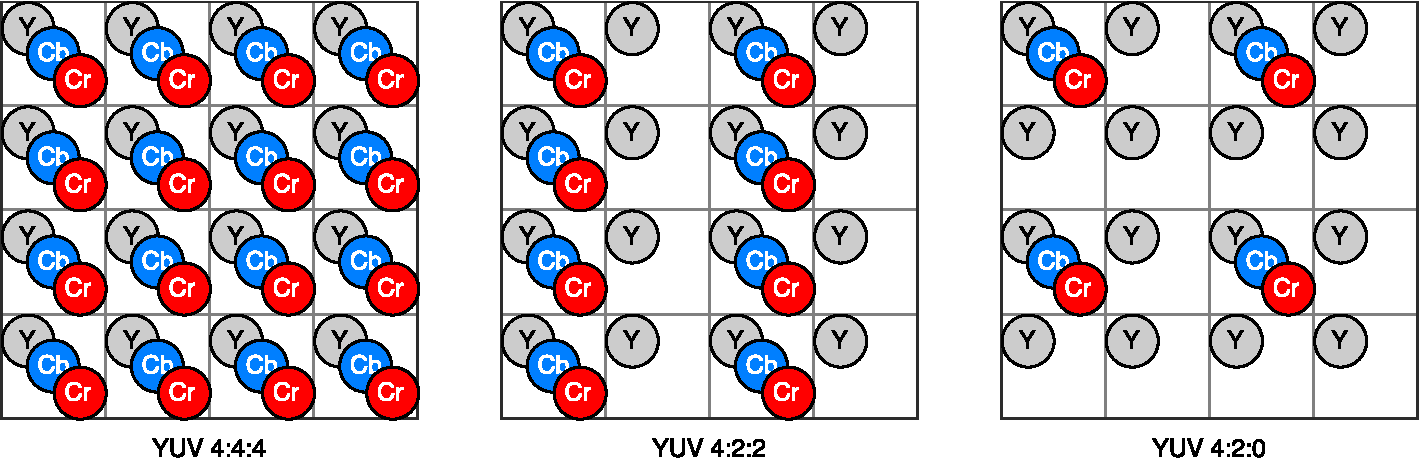
\includegraphics[bb=0 0 681 222,width=14cm]{img/yuv-pixel-structure.pdf}
    \end{center}
    \caption{YUVのピクセルあたりの色情報の構造}
    \label{fig:yuv-pixel-structure}
\end{figure}

% YUVのピクセルあたりの色情報の構造を、図\ref{fig:yuv-pixel-structure}に示す。

YUV 4:4:4では、輝度信号、色差信号共に1ピクセル毎である。
YUV 4:2:2では、輝度信号は1ピクセル毎、色差信号は2ピクセル毎であり、同じ色深度のYUV 4:4:4と比べ、帯域はおよそ2/3となる。
YUV 4:2:0では、輝度信号は1ピクセル毎、色差信号は4ピクセル毎であり、同じ色深度のYUV 4:2:2と比べ、帯域はおよそ3/4となり、同じ色深度のYUV 4:4:4と比べ、帯域はおよそ1/2となる。

なお、図\ref{fig:yuv-pixel-structure}で示した、UV成分であるCb、Crの色のサンプリング方法は、伝送方式の規格によって定められている。

\section{インターフェース}
\label{sec:interface}

\subsection{VGA}
VGA(Video Graphics Array)は、IBMが発表したアナログ映像信号の伝送規格、または、同社が開発したVGA表示回路用のチップのことを指す。
DE-15コネクタを使用し、赤、緑、青、垂直同期、水平同期の5つのアナログ信号で映像を伝送することができる。
DDC(VESA Display Data Channel)信号を使用することで、接続機器の対応する解像度を送信することができ、最近では1080pの映像を伝送する機器も多い。
PCでの映像出力方式として普及したが、アナログ信号であることや、音声伝送の手段が別途必要となるため、HDMIやDisplayPortなどのインターフェースに移行が進んでいる。

\subsection{DisplayPort}
DisplayPortは、VESA\footnote{Video Electronics Standards Association ビデオ周辺機器に関する業界標準化団体}によって標準化された映像伝送規格であり、主に超解像度向けのインターフェースとして普及している。
DisplayPort 1.3からは、32.4 Gbpsのデータレートに対応し、8K映像の伝送にも対応している。

\subsection{DVI}
DVI(Digital Visual Interface)は、VESA\footnote{Video Electronics Standards Association ビデオ周辺機器に関する業界標準化団体}によって標準化された デジタル映像信号の伝送規格である。
物理層として、Silicon Imageが開発したTMDS(Transition Minimized Differential Signaling)を使用している。
TMDSは、データの3チャネルとクロックの1チャネルを備えた4つのツイストペアケーブルで構成され、主に高速シリアル通信で使用されている。
TMDSでは、データの8b/10b符号化が行われ、データレートは20\%のロスとなるが、DC成分の偏りを押さえ、ブランキング区間などでもI/Oの遷移を増やしてデータの境界検出を用意にしている。

\subsection{HDMI}
HDMI(High-Definition Multimedia Interface)は、映像、音声をデジタル信号で伝送する通信インターフェースの規格である。
DVIを基に、音声伝送機能や著作権保護機能を加えたものであり、物理層はDVIと同じTMDSを使用している。

HDMIのシステム構成は大きく分けて、映像を送る機器(Source)、映像を受け取る機器(Sink)、ケーブルの3つに分類することができる。

\begin{figure}[htbp]
    \begin{center}
        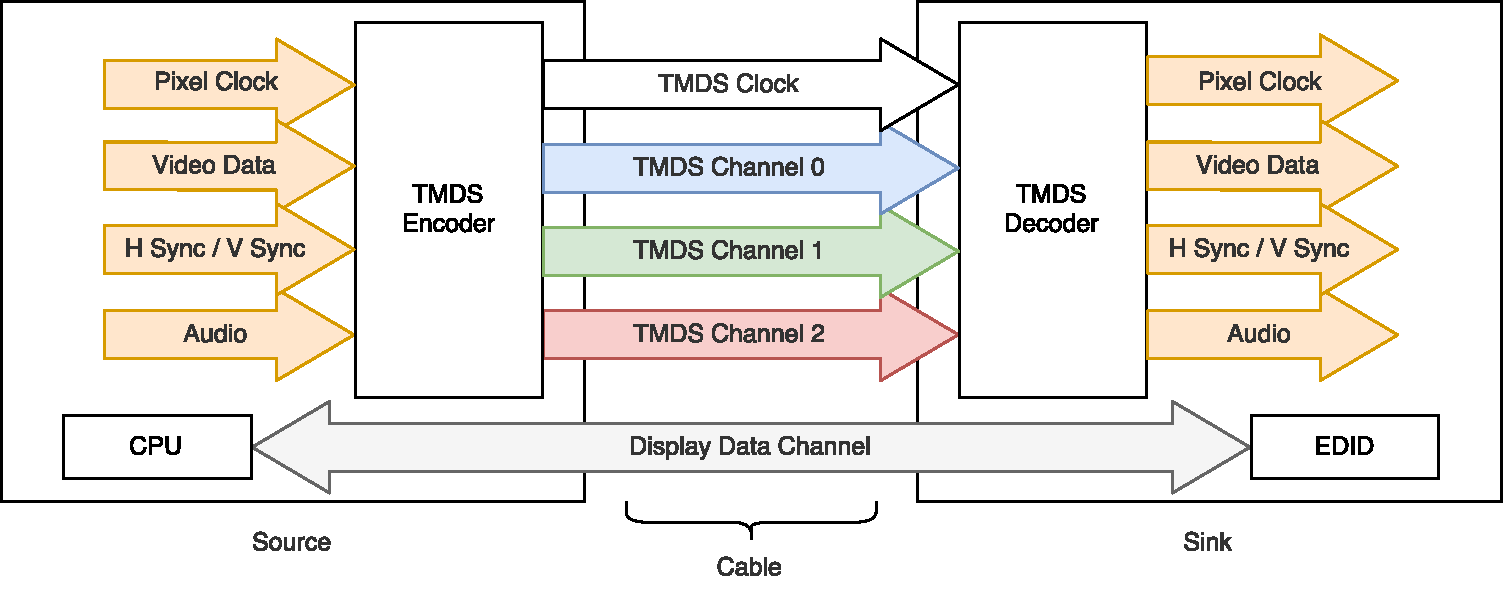
\includegraphics[bb=0 0 721 283,width=15cm]{img/hdmi-spec-structure.pdf}
    \end{center}
    \caption{HDMIブロックダイアグラム}
    \label{fig:hdmi-spec-structure}
\end{figure}

HDMI 2.0では、帯域を18Gbpsに拡大し、4K@60pに対応している。
また、CES 2017に合わせ、HDMI 2.1が発表され、帯域を48Gbpsに拡大し、8K@60pに対応した。

\begin{table}[htbp]
  \caption{HDMI 1.4と2.0での4K(3840x2160)映像の対応状況}
  \label{tb:video-bandwidth}
  \begin{center}
  \begin{tabular}{c|c|c|c}
    \hline
      フレームレート & ピクセルあたりの色深度 & HDMI 1.4 & HDMI 2.0\\\hline\hline
    \multirow{4}{*}{30Hz} &
        24bit & 対応   & 対応 \\\cline{2-4}
      & 30bit & 対応   & 対応 \\\cline{2-4}
      & 36bit & 対応   & 対応 \\\cline{2-4}
      & 48bit & 非対応 & 対応 \\\hline
    \multirow{4}{*}{60Hz} &
        24bit & 非対応 & 対応  \\\cline{2-4}
      & 30bit & 非対応 & 対応  \\\cline{2-4}
      & 36bit & 非対応 & 対応  \\\cline{2-4}
      & 48bit & 非対応 & 非対応 \\\hline
  \end{tabular}\end{center}
\end{table}

HDMI 1.4\cite{hdmi-spec-1-4}では、RGB、YCbCr 4:4:4、YCbCr 4:2:2の色空間がサポートされている。
HDMI 2.0\cite{hdmi-spec-2-0}では、4K解像度向けにYCbCr 4:2:0の色空間がサポートされた。
YCbCr 4:2:0によるピクセルエンコーディングの規格では、YCbCr 4:2:2と比べ、1/2のデータレートで転送することが可能となった。
これにより、一部の機器では4K解像度への対応をソフトウェアだけで行なうことが可能である。

YCbCr 4:4:4、YCbCr 4:2:2のTMDSデータのマッピングを、図\ref{fig:hdmi-spec-yuv-444}と図\ref{fig:hdmi-spec-yuv-422}に示す。

\begin{figure}[htbp]
    \begin{center}
        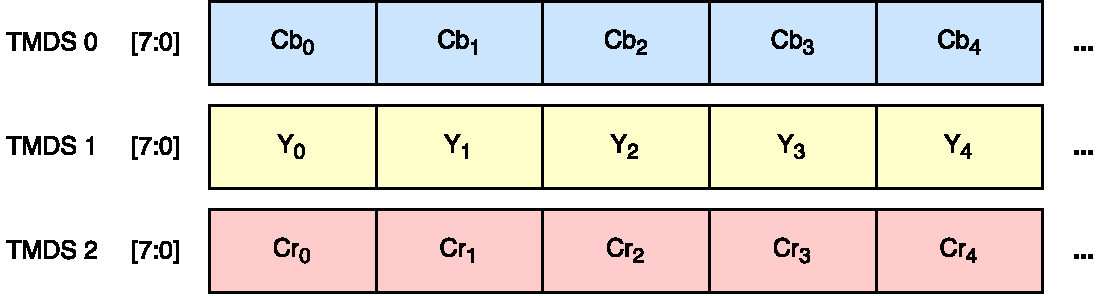
\includegraphics[bb=0 0 531 141,width=13.926cm]{img/hdmi-spec-yuv-444.pdf}
    \end{center}
    \caption{HDMI 1.4 で定義されている YCbCr 4:4:4 におけるTMDSマッピング}
    \label{fig:hdmi-spec-yuv-444}
\end{figure}

\begin{figure}[htbp]
    \begin{center}
        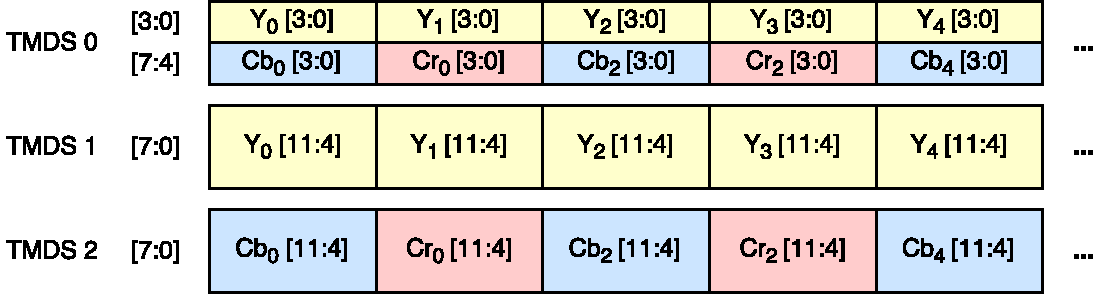
\includegraphics[bb=0 0 531 141,width=13.926cm]{img/hdmi-spec-yuv-422.pdf}
    \end{center}
    \caption{HDMI 1.4 で定義されている YCbCr 4:2:2 におけるTMDSマッピング}
    \label{fig:hdmi-spec-yuv-422}
\end{figure}

\ref{sec:colorspace}節では、同じ色深度の場合YUV 4:2:2はYUV 4:4:4と比べ2/3となると述べたが、HDMI 1.4で定義されているYCbCr 4:2:2では、1ピクセルあたりの色深度は変わらず、YおよびCbCrのサンプリング解像度が8bitから12bitになる。
そのため、HDMIでは色空間のYCbCr 4:4:4、YCbCr 4:2:2のどちらであっても帯域には影響しない。

\newpage
YCbCr 4:2:0のTMDSデータのマッピングを、図\ref{fig:hdmi-spec-yuv-420}に示す。

\begin{figure}[htbp]
    \begin{center}
        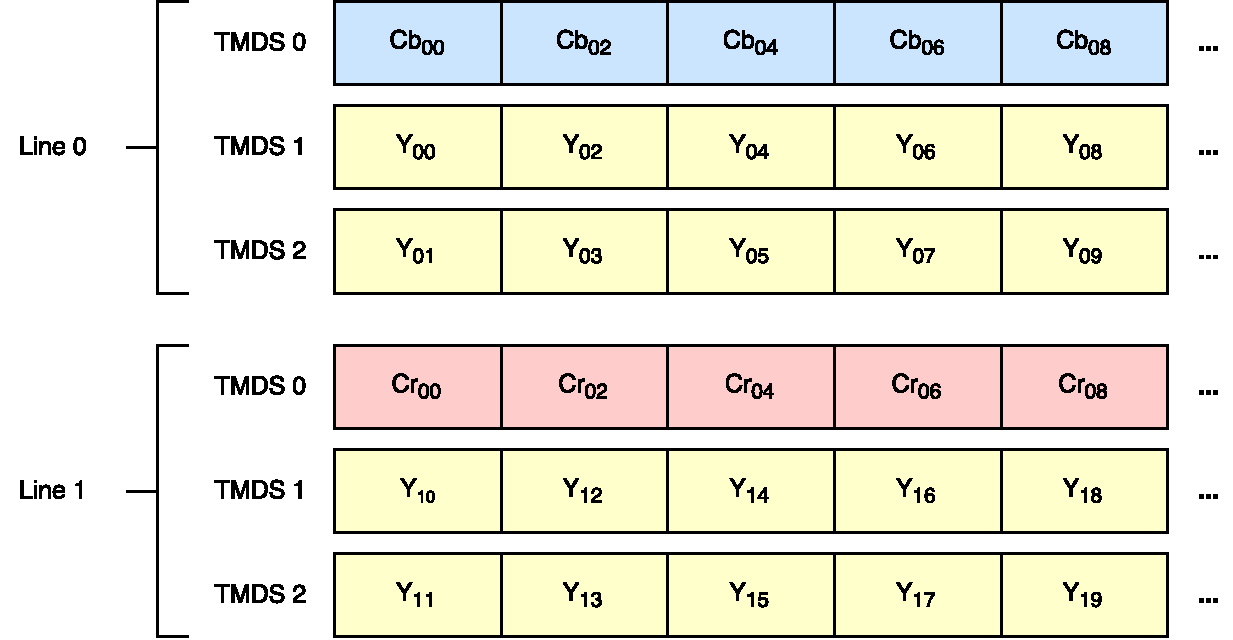
\includegraphics[bb=0 0 591 306,width=15.5cm]{img/hdmi-spec-yuv-420.pdf}
    \end{center}
    \caption{HDMI 2.0 で定義されている YCbCr 4:2:0 におけるTMDSマッピング}
    \label{fig:hdmi-spec-yuv-420}
\end{figure}

HDMIでは、24bitの他に、30bit、36bit、48bitの色深度に対応しているが、YCbCr 4:2:0では、24bitのみの対応である。

\subsection{SDI}

SDI(Serial Digital Interface)は、SMPTE\footnote{米国映画テレビ技術者協会}によって標準化された映像伝送規格であり、主に業務機器向けの規格である。

同軸ケーブルを使用しているため、HDMIと比べて距離に対する減衰が少なく、HD-SDIでは、およそ100m遠方に伝送することができる。
BNC端子を使用することが一般的であり、抜け落ち防止のためのロック機能がるため、放送局や中継現場で使われる。

解像度や帯域に応じて、SD-SDI、HD-SDI、3G-SDI、6G-SDI、12G-SDIなど複数の規格が定められている。
また、4K・8K映像を伝送するために、HD-SDIや3G-SDIを2本1組や4本1組で使用して伝送する規格も定められている。

\section{帯域}
\label{sec:bandwidth}
帯域は解像度の他にも、インターレース、色空間、色深度により変化する。
また、伝送するインターフェースの規格によっても、物理層での扱いにより若干の違いがある。
ここでは、HDMIで色深度を8bitとした場合の解像度、フレームレート、色空間別に見たピクセルクロック、データレートを表\ref{tb:video-bandwidth}に示す。

% 1920x1080p/60 2200x1125 148.5 SMPTE 274M
% 1Channel = 2200 * 1125 * 3 * 8 * 60 * 1.25/3

同期区間を含めた垂直ピクセルを$p_w$、水平ピクセルを$p_h$、ピクセルあたりのビット数を$b$、フレームレートを$f$としたとき、HDMIのデータレート$r$は次のようにして求めることができる。
HDMIの物理層であるTMDSでは、8b/10b変換が行われるため、データレートとしては1.25倍となることに注意していただきたい。

\[ r=1.25bfp_wp_h \]

\begin{table}[htbp]
  \caption{解像度、フレームレート、色空間によるHDMIのデータレートの変化}
  \label{tb:video-bandwidth}
  \begin{center}
  \begin{tabular}{c|c|c|c|c}
    \hline
    解像度     & フレームレート & 色空間  & ピクセルクロック & データレート  \\\hline\hline
    3840x2160 & 60p          & RGB    & 594MHz        & 17.82 Gbps  \\\hline
    3840x2160 & 60p          & YUV422 & 594MHz        & 17.82 Gbps  \\\hline
    3840x2160 & 60p          & YUV420 & 297MHz        & 8.91 Gbps   \\\hline
    3840x2160 & 30p          & RGB    & 297MHz        & 8.91 Gbps   \\\hline
    3840x2160 & 30p          & YUV422 & 297MHz        & 8.91 Gbps   \\\hline
    1920x1080 & 60p          & RGB    & 148.5MHz      & 4.455 Gbps  \\\hline
    1920x1080 & 60p          & YUV422 & 148.5MHz      & 4.455 Gbps  \\\hline
    1920x1080 & 60i          & RGB    & 74.25MHz      & 2.2275 Gbps \\\hline
    1920x1080 & 60i          & YUV422 & 74.25MHz      & 2.2275 Gbps \\\hline
  \end{tabular}\end{center}
\end{table}

\section{IP伝送規格}
Video over IPにおける映像のIP伝送規格は、SMPTE 2022とNMIが主流となっている\cite{kodera-interbee2016}。
しかし、その他にも多くの規格が提唱され、市場ではどの規格で統一されるかが静観されている。

IP伝送規格は、SDIなどの標準化を行っているSMPTEや、映像制作現場などの機器を制作している会社が製品とともに規格化を行う事が多い。
この節では、抜粋して幾つかのIP伝送規格について解説する。

\subsection{SMPTE 2022}
SMPTE 2022は、SMPTEが提唱、標準化したIP伝送規格であり、表\ref{tb:smpte2022-abstract}に示す7つの規格に分かれている。

\begin{table}[htbp]
  \caption{SMPTE 2022の7つの規格の概要}
  \label{tb:smpte2022-abstract}
  \begin{center}
  \begin{tabular}{c|l}
    \hline
    規格          & 概要 \\\hline\hline
    SMPTE 2022-1 & IP伝送でのリアルタイムビデオ/オーディオ転送のFEC訂正 \\\hline
    SMPTE 2022-2 & IP伝送での固定ビットレートMPEG-2 TSの単方向転送 \\\hline
    SMPTE 2022-3 & IP伝送での可変ビットレートMPEG-2 TSの単方向転送 \\\hline
    SMPTE 2022-4 & IP伝送での非ピース単位の可変ビットレートMPEG-2ストリームの単方向転送 \\\hline
    SMPTE 2022-5 & IP伝送での高ビットレートメディア信号の伝送のための前方誤り訂正 \\\hline
    SMPTE 2022-6 & IP伝送でのネットワークを介した高ビットレートメディア信号の伝送 \\\hline
    SMPTE 2022-7 & IPデータグラムのシームレスな保護スイッチング \\\hline
  \end{tabular}\end{center}
\end{table}

SMPTE 2022-1/2/3/4では、MPEG2圧縮をベースとしたIP伝送について規格化され、SMPTE 2022-5/6では、非圧縮でありSDIのペイロードを基としたIP伝送について規格化されている。

\subsection{SMPTE 2110}
SMPTE 2110は、SMPTEが制定中の規格であり、VSF(Video Services Forum)に提出されたTR03、TR04の内容を取り込んでいる。

SMPTE 2022-5/6ではSDIのペイロードを基としているため、IPパケットにする際にはSDIをカプセル化している。
そのため、映像と音声データをIPレイヤーから識別することができず、制御に利用しにくいなどの問題がある。
この問題を回避するため、SMPTE 2110では、ビデオデータの伝送にはRFC 4175\cite{rfc4175}のRTP、音声データの伝送にはAES 67を使用するなど、より効果的なIP伝送規格になるよう設計されている。

\subsection{NMI ネットワーク・メディア・インターフェース}
NMI\cite{sony-nmi}は、ソニービジネスソリューションが提唱、規格化したIP伝送規格である。

非圧縮ではなく、低遅延高画質のコーデックであり、Visually LosslessなLLVC\cite{smpte-rdd-34}によって圧縮されている。
また、機器間の同期にはナノ秒レベルの高精度同期が行える、SMPTE ST2059を使用している。

\subsection{NDI ネットワーク・デジタル・インターフェース}
NDI\cite{newtek-ndi}は、NewTekが提唱、開発したオープンなIP伝送規格である。

多くのIP伝送規格は商用向けであり、詳細な仕様はオープンになっていないが、NDIではSDKやプラグインなどを公開し、ユーザーを集めている。

\section{まとめ}
TBD
% また、各インターフェースでは、実際の映像のデータだけではなく、同期区間や物理層による8b/10b変換などによりデータ量が増加することも明らか

\chapter{NG-HDMI-TS}
\label{chap:network-transmission}

% \section{仮説}
映像のIP伝送については既に多くの先行研究があり、映像を拠点間などで伝送するための製品なども存在している。

しかし、本論文では、拠点間のIP伝送だけにとどまらず、拠点内の設備までもをIP伝送することをテーマとしている。
拠点内の設備として、カメラやスイッチャー、ディスプレイなどの拠点内の設備までもをIP伝送で行う、Video over IP化にするというテーマである。

そのため、実際に制作の現場にIP伝送を普及させた際に、現在の伝送方法の課題が解決でき、IP伝送を利用することができるのかについて検証する。

% \subsection{Ethernetを活用するメリット}

\ref{chap:introduction}章で、述べた通り、ネットワークを活用することによって活かせるメリットは以下の3つである。

\begin{itemize}
  \item 1本のケーブルで複数や双方向の映像が可能
  \item 伝送スピードの向上
  \item コストダウン
\end{itemize}

しかし、Ethernetを利用するためにはデメリットがある

輻輳
導入コストの

また、映像伝送における重要なポイントは以下の3つである。

\begin{itemize}
  \item 画質、音質の劣化がない
  \item 伝送遅延を一定以下にする必要がある
  \item 安定性がある
\end{itemize}

また、IP伝送のメリットは以下の点である。

\begin{itemize}
  \item ユニキャスト、ブロードキャストが行える
\end{itemize}

これらの点において評価を行う。

% 1
\section{映像制作現場で求められるIP伝送装置の要件}
% ファイルベースの映像編集では、ネットワークストレージを活用した環境
% しかし、ライブでは、同軸ケーブルを利用してきました。これは、映像や音声を安定的に伝送することが求められているからです。

リアルタイムの映像伝送では、前出の通り同軸ケーブルを使用することが一般的である。

映像や音声を安定的に伝送することが出来、
現場での取り回しの氏易さ
IP

中継でのIP伝送では、ある程度の遅延[要出典]は許容することができる。
屋外での中継で、外にいるリポーターと局内にいるキャスターとの音声に遅延があり、やり取りに間があることがある。
これは、映像

しかし、拠点内でのIP伝送であれば、映像と音声が同期している必要があり、各カメラごとに遅延が異なるようではいけない。

\section{遅延}

\section{調査}

% \begin{figure}[htbp]
%   \begin{minipage}{0.5\hsize}
%     \begin{center}
%         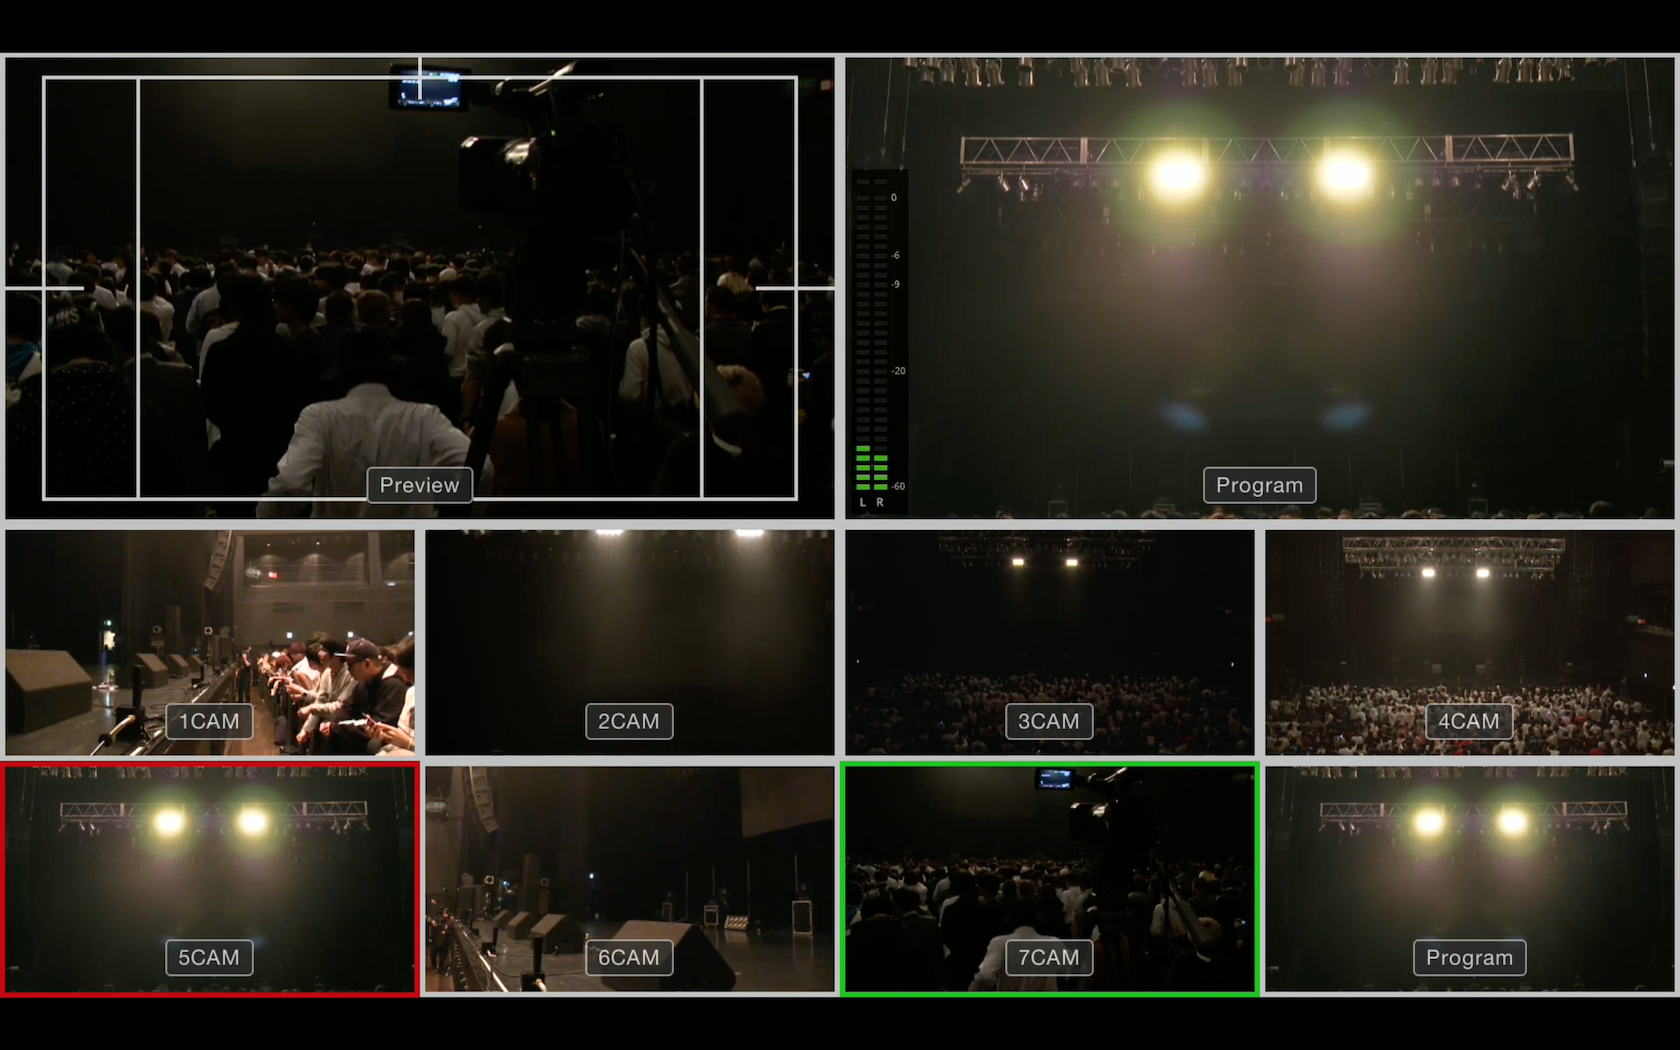
\includegraphics[bb=0 0 1680 1050,width=8cm]{img/mv-delay-actual.png}
%     \end{center}
%     \caption{TED HDMI 2.0 FMCカード (TB-FMCH-HDMI4K)}
%     \label{fig:ted-4k-fmc-card}
%   \end{minipage}
%   \begin{minipage}{0.5\hsize}
%     \begin{center}
%         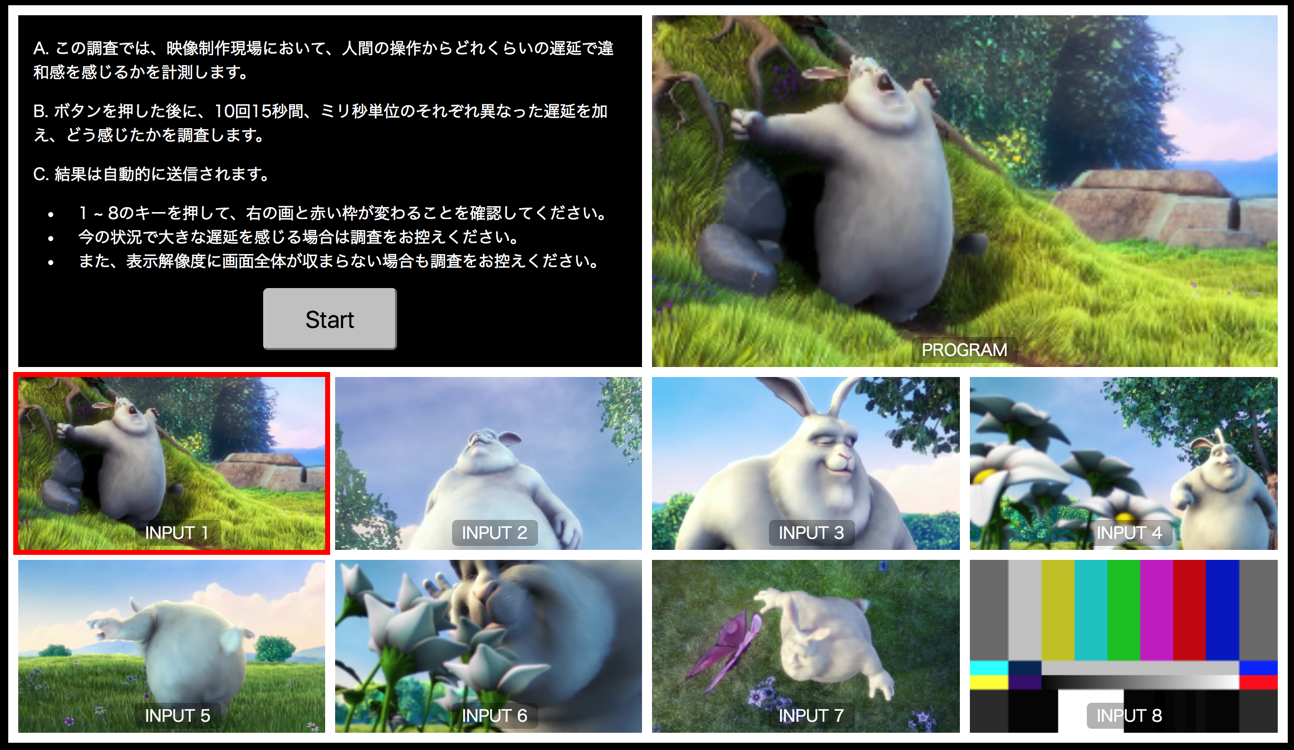
\includegraphics[bb=0 0 1294 750,width=8cm]{img/mv-delay-virtual.png}
%     \end{center}
%     \caption{TED HDMI 2.0 FMCカード (TB-FMCH-HDMI4K)}
%     \label{fig:ted-4k-fmc-card}
%   \end{minipage}
% \end{figure}

\begin{figure}[htbp]
  \begin{center}
    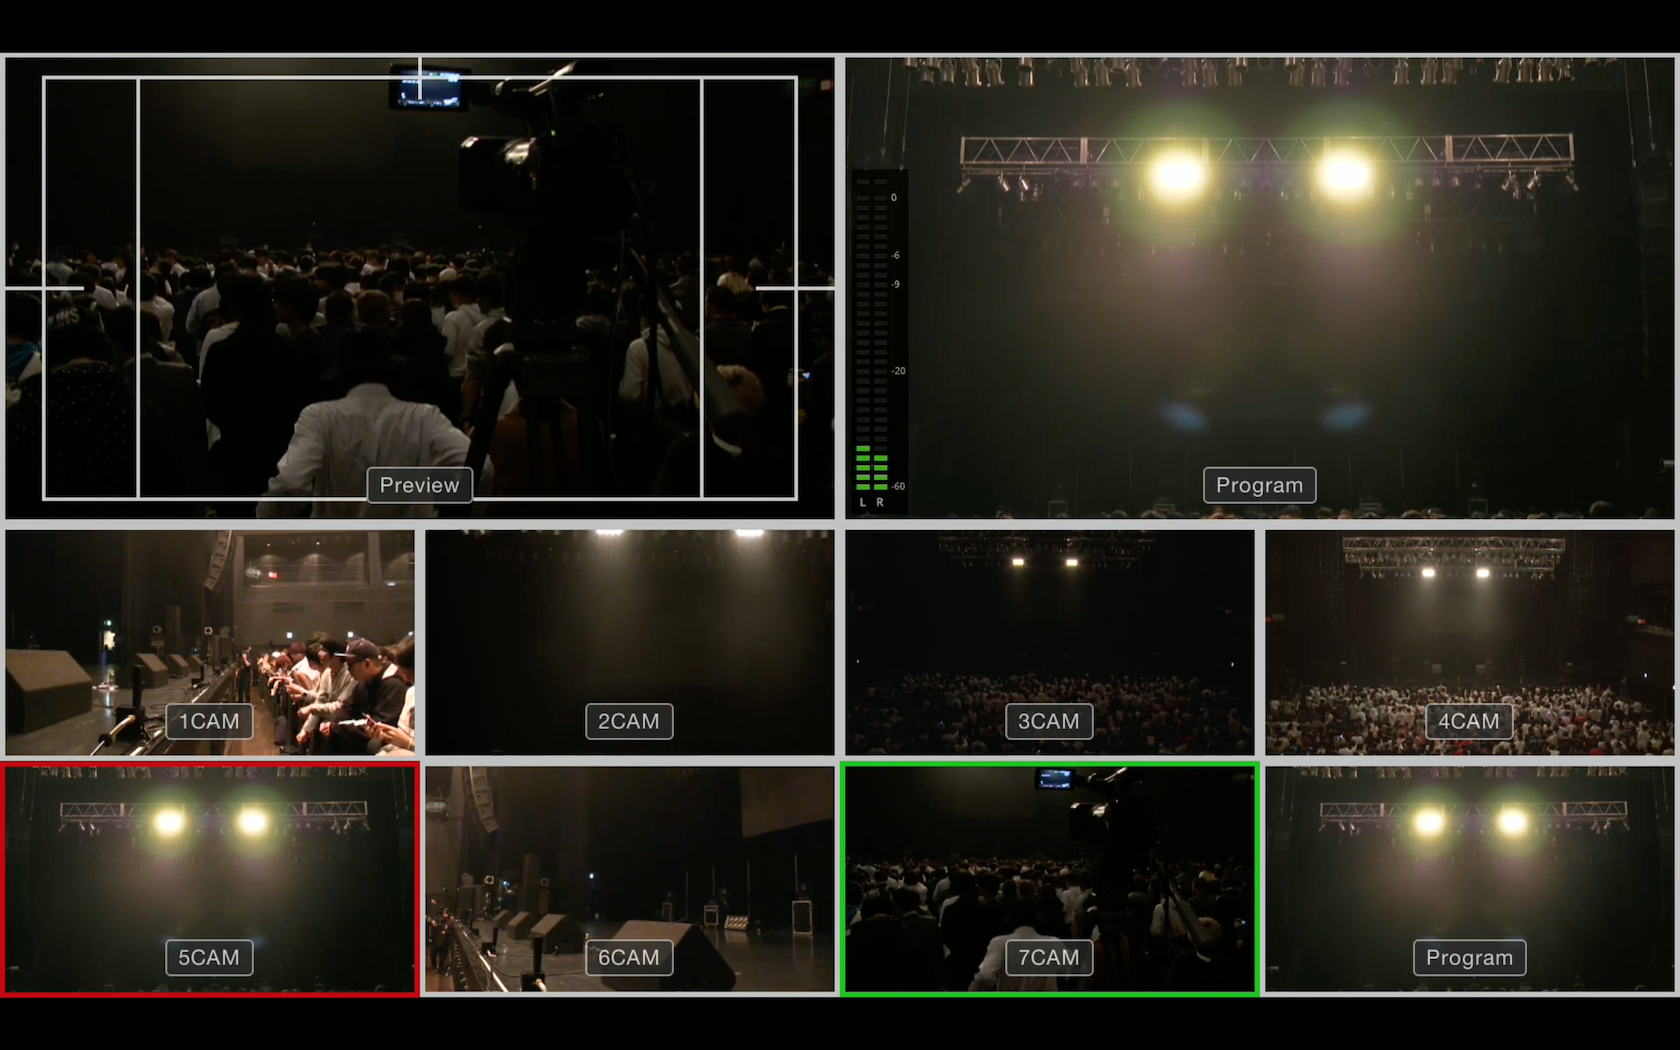
\includegraphics[bb=0 0 1680 1050,width=8cm]{img/mv-delay-actual.png}
  \end{center}
  \caption{}
  \label{fig:ted-4k-fmc-card}
\end{figure}
\begin{figure}[htbp]
  \begin{center}
    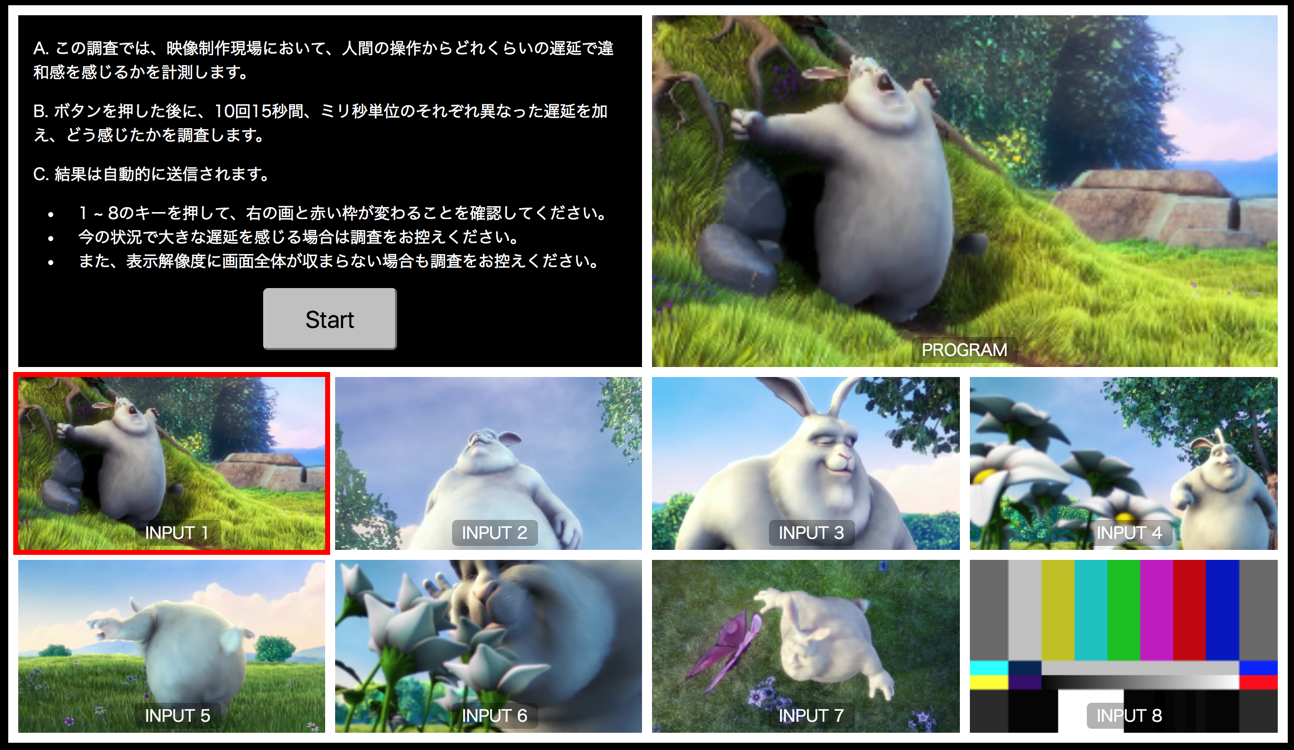
\includegraphics[bb=0 0 1294 750,width=8cm]{img/mv-delay-virtual.png}
  \end{center}
  \caption{今回の実験で使用したWebページ}
  \label{fig:ted-4k-fmc-card}
\end{figure}

\section{目的}

映像の制作の現場では、符号化・複合などによる映像の遅延を抑えることや、画質をそのまま伝送することがしばしば求められます。
このような背景から、4K映像を非圧縮のままIP伝送する技術の実証実験と、現場においてIP伝送を利用する際に問題となる点を洗い出します。?

% \section{構成}

\chapter{システムの設計・実装}
\label{chap:implementation}

本章では、\ref{chap:video-production}章で述べた、映像制作現場におけるIP伝送装置について評価するため、4K映像を非圧縮でIPで伝送するシステムであるNG-HDMI-TSをハードウェアで実装したことについて実装の解説をする。

\section{実装の概要}

IP伝送装置は、Xilinx KC705 評価ボード\cite{xilinx-kc705}、HDMIインターフェースカードであるTED HDMI 2.0 FMCカード\cite{ted-hdmi4k}を使用した。
本実装の構成を図~\ref{fig:fpga-implement-flow}に示す。

\begin{figure}[htbp]
  \begin{center}
    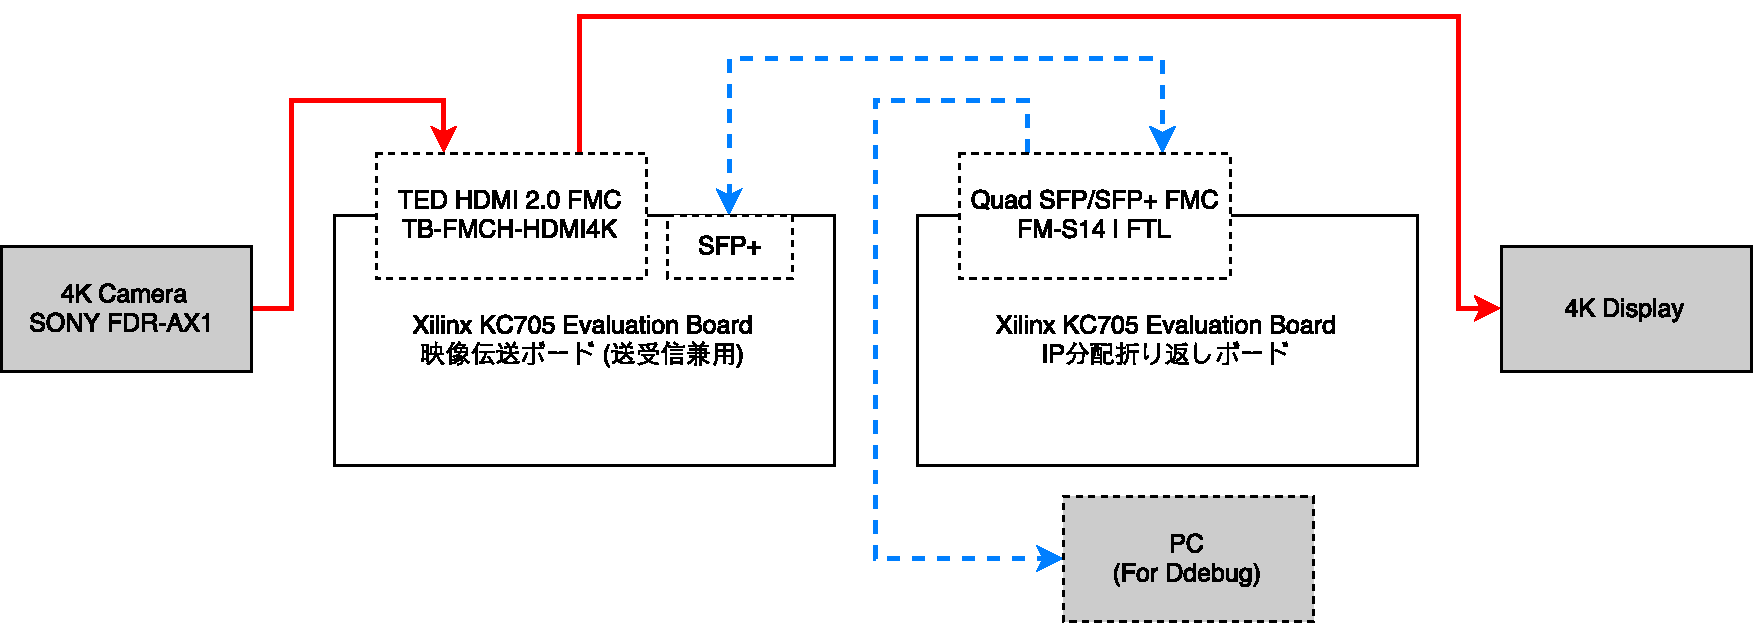
\includegraphics[bb=0 0 841 299,width=15.5cm]{img/fpga-implement-flow.pdf}
  \end{center}
  \caption{ハードウェアによる実装の構成}
  \label{fig:fpga-implement-flow}
\end{figure}

\begin{figure}[htbp]
  \begin{center}
    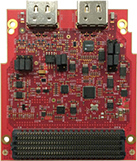
\includegraphics[bb=0 0 137 161,width=4cm]{img/ted-4k-fmc-card.jpg}
  \end{center}
  \caption{TED HDMI 2.0 FMCカード (TB-FMCH-HDMI4K)}
  \label{fig:ted-4k-fmc-card}
\end{figure}

% \begin{table}[htbp]
%   \caption{ハードウェアによる実装を行ったPCの構成}
%   \label{tb:software-specification}
%   \begin{center}
%   \begin{tabular}{c||c}
%     \hline
%     ソフトウェア  & Vivado 2016.2 \\\hline
%   \end{tabular}\end{center}
% \end{table}

今回の構成では、IP伝送装置とは別に1台のXilinx KC705 評価ボード、Quad SFP/SFP+カードを用いて、送信したIPパケットを折り返しする装置を使用した。
IPパケットを折り返しする装置について、IP伝送装置と直接の関係はないため、ここでの解説は割愛する。

本実装では、論理合成ツールとしてXilinx Vivado 2016.2を使用した。また、開発言語としてVerilog HDLを使用した。

\section{FPGAの回路設計}

本実装は、Xilinxが提供しているKintex-7シリーズ向けのHDMI 2.0のリファレンス実装であるxapp1287\cite{xilinx-xapp1287}をベースとしている。
Xilinxの提供するIPである10 Gigabit Ethernet Subsystem\cite{xilinx-pg157}、Video PHY Controller\cite{xilinx-pg230}、HDMI 1.4/2.0 Transmitter Subsystem\cite{xilinx-pg235}、及び、HDMI 1.4/2.0 Receiver Subsystem\cite{xilinx-pg236}、FIFO Generator\cite{xilinx-pg057}が使用されている。
本研究のために新たに実装をした箇所は、これらのIPに対してデータを受け渡しするモジュールとそのモジュールを含んだEthlogic Subsystemである。
FPGAの回路全体のブロックダイアグラムを図~\ref{fig:fpga-whole-diagram}に示す。なお、IP伝送装置に関係するモジュールのみを掲載している。

\begin{figure}[htbp]
  \begin{center}
    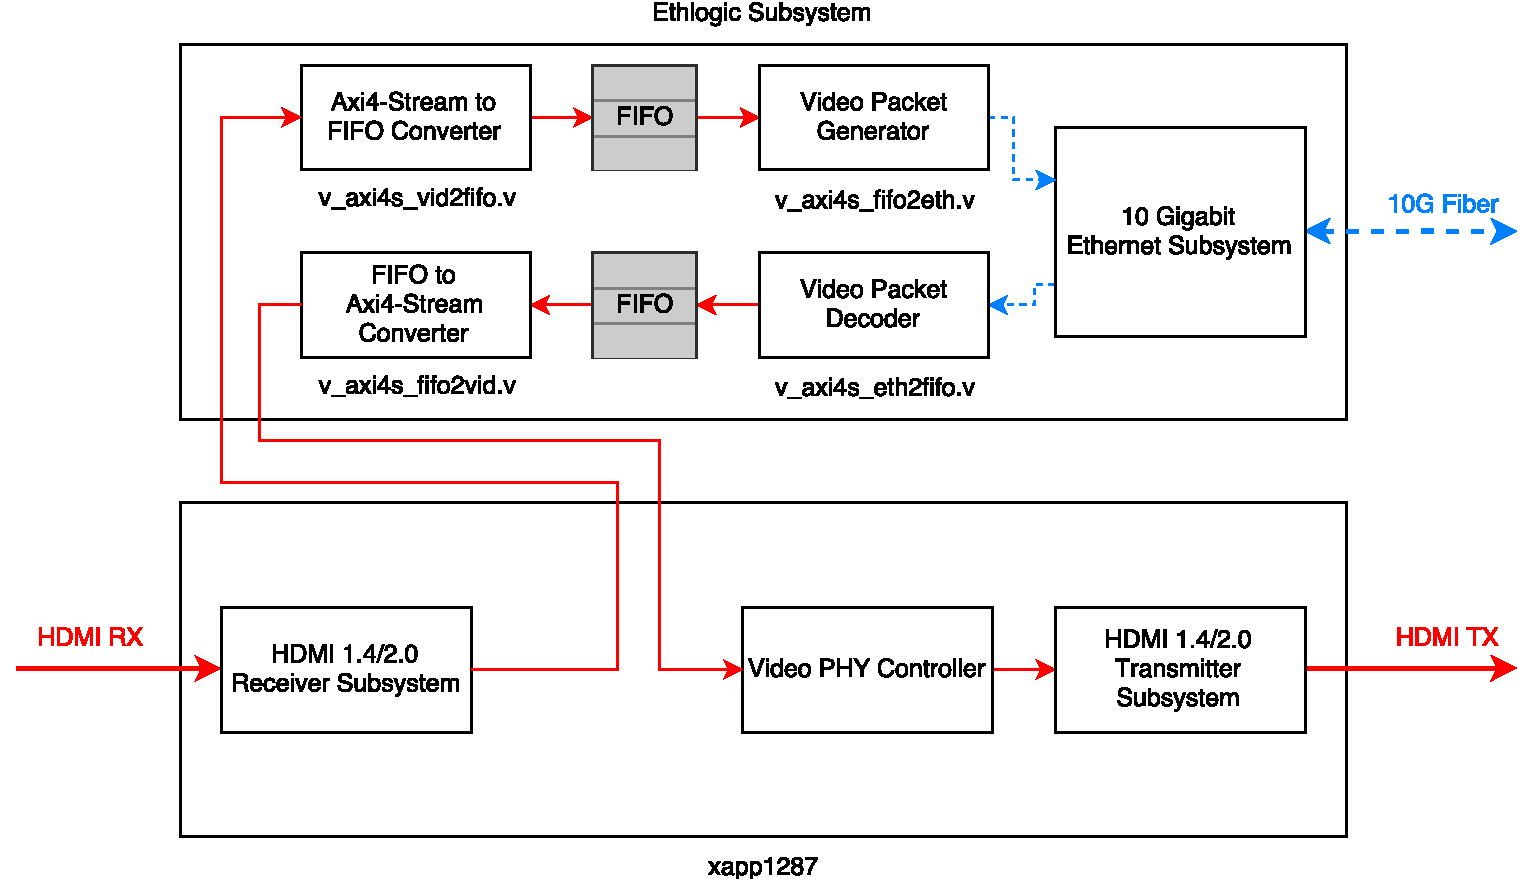
\includegraphics[bb=0 0 738 423,width=15.5cm]{img/fpga-whole-diagram.pdf}
  \end{center}
  \caption{FPGA回路全体のブロックダイアグラム}
  \label{fig:fpga-whole-diagram}
\end{figure}

受信側と送信側で、10 Gigabit Ethernet SubsystemとVideo Processing Subsystem間の受け渡しを行うため、表~\ref{tb:fpga-implement-modules}に示す4つのモジュールを実装した。

\begin{table}[htbp]
  \caption{10 Gigabit Ethernet Subsystem、及び、Video Processing Subsystemの接続のために実装したモジュール}
  \label{tb:fpga-implement-modules}
  \begin{center}
  \begin{tabular}{c|p{12cm}}
    \hline
    Name               & Description \\\hline\hline
    v\_axi4s\_eth2fifo.v & Ethernet Subsystemのクロックで、Ethernet Subsystemから送られてきた映像データをFIFOに書き込むモジュール \\\hline
    v\_axi4s\_fifo2eth.v & Ethernet Subsystemのクロックで、FIFOから読み込んだの映像データをEthernet Subsystemに送るモジュール \\\hline
    v\_axi4s\_vid2fifo.v & Video Processing Subsystemのクロックで、Video Processing Subsystemから送られてきた映像データをFIFOに書き込むモジュール \\\hline
    v\_axi4s\_fifo2vid.v & Video Processing Subsystemのクロックで、FIFOから読み込んだの映像データをVideo Processing Subsystemに送るモジュール \\\hline
  \end{tabular}\end{center}
\end{table}

10 Gigabit Ethernet Subsystemの基準クロックは64bit幅の設定で156.25MHzとなり、Video Processing Subsystemの基準クロックは300MHzとなる。
互いの基準クロックが異なるため、データをそのまま受け渡しすることはできない。

この問題を解決するため、読み書きで独立したクロックに対応したIndependent Clocking FIFOをFIFO Generatorで作成する。
今回のIP伝送装置の送信側で用いた、FIFOのモジュールを図~\ref{fig:fpga-independent-clocking-fifo}に示す。

\begin{figure}[htbp]
  \begin{center}
    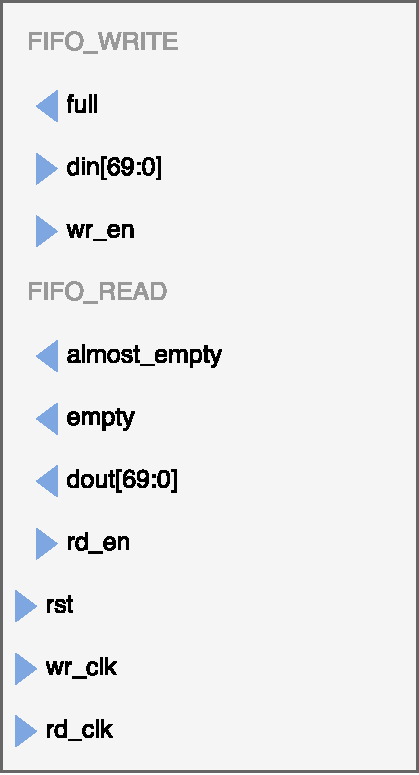
\includegraphics[bb=0 0 201 371,width=4cm]{img/fpga-independent-clocking-fifo.pdf}
  \end{center}
  \caption{Independent Clocking FIFO}
  \label{fig:fpga-independent-clocking-fifo}
\end{figure}

読み書きで独立したクロックの他に、入出力のデータ幅が異なっており、入力のデータ幅は35bit、出力のデータ幅は倍の70bitとなっている。理由は後述する。
Video Processing Subsystemは300MHzで35bitのデータを書き込み、10 Gigabit Ethernet Subsystemは156.25MHzのデータを読み込む。
10 Gigabit Ethernet Subsystemのクロックが早いため、FIFOがフル状態になることはない。
また、almost\_emptyフラグを使用しており、emptyになる1クロック前に知ることが可能である。

送信側のモジュールの接続を図~\ref{fig:fpga-video-ethernet-diagram}に示す。

\begin{figure}[htbp]
  \begin{center}
    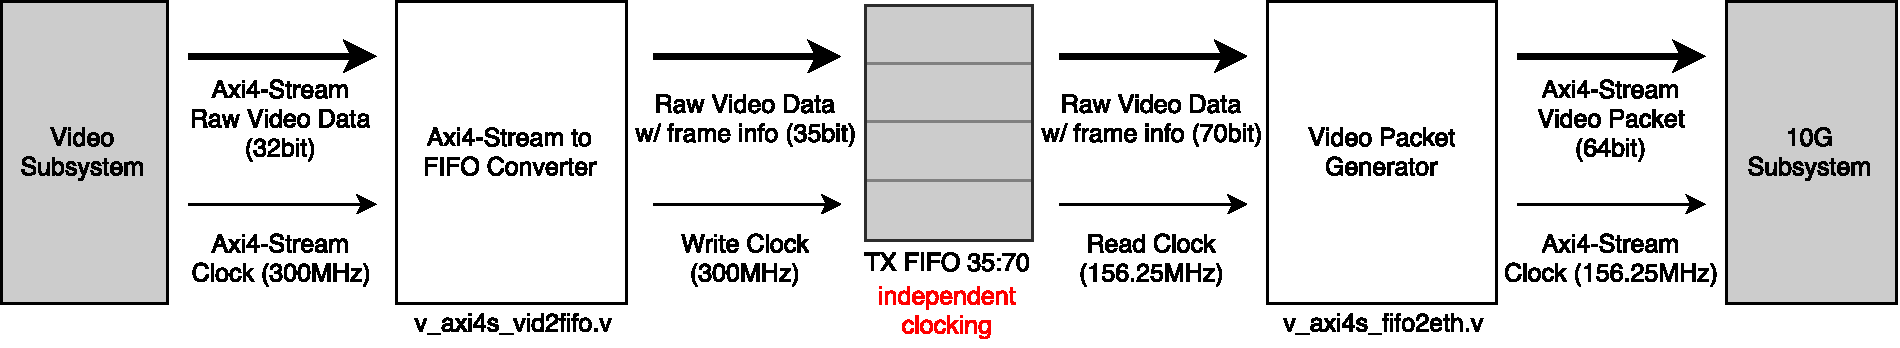
\includegraphics[bb=0 0 911 166,width=15.5cm]{img/fpga-video-ethernet-diagram.pdf}
  \end{center}
  \caption{Video Stream to Ethernet Packet Subsystem Diagram}
  \label{fig:fpga-video-ethernet-diagram}
\end{figure}

受信側のモジュールの接続を図~\ref{fig:fpga-ethernet-video-diagram}に示す。

\begin{figure}[htbp]
  \begin{center}
    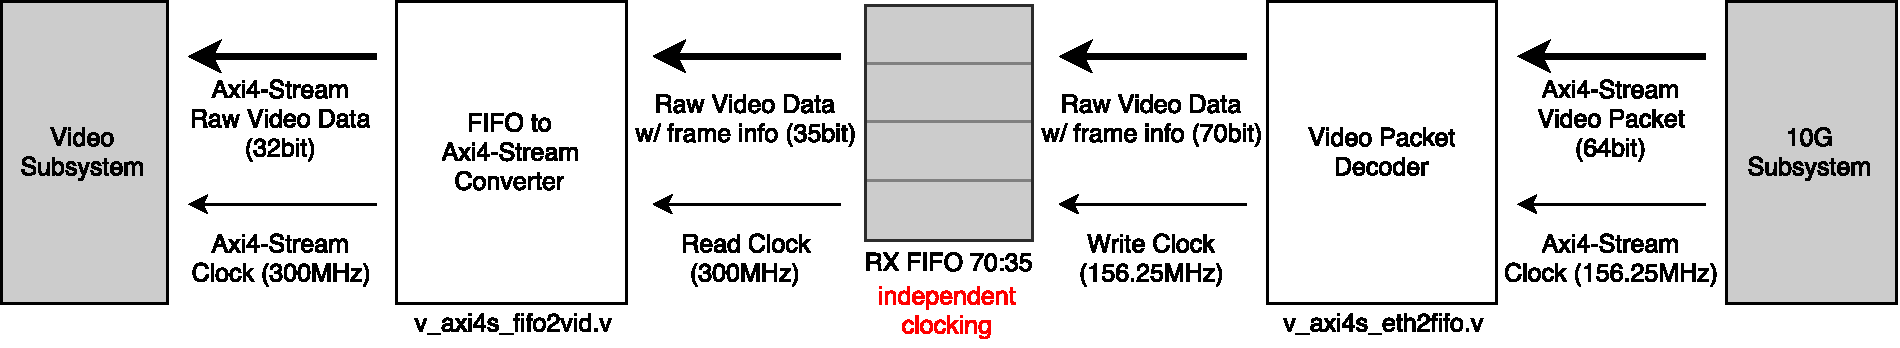
\includegraphics[bb=0 0 911 166,width=15.5cm]{img/fpga-ethernet-video-diagram.pdf}
  \end{center}
  \caption{Ethernet Packet to Video Stream Subsystem Diagram}
  \label{fig:fpga-ethernet-video-diagram}
\end{figure}

Video Processing Subsystemが出力するAxi4-Streamのtdataは映像データを表し、有効データ幅は32bitである。
また、表~\ref{tb:fpga-axi4-stream}に示すとおり、tlastがラインの終了、tuserがフレームの開始を表す。
FIFOに映像データだけを書き込んだ場合、ラインの終了、フレームの開始のタイミングが失われることとなる。
この問題を解決するため、FIFOにはAxi4-Streamのtdataの他に、tlast、tuser、tvalidも書き込む。

\begin{table}[htbp]
  \caption{Video Processing SubsystemのAxi4-Streamインターフェース}
  \label{tb:fpga-axi4-stream}
  \begin{center}
  \begin{tabular}{l|c|l}
    \hline
    Name   & Width     & Description \\\hline\hline
    tdata  & 3*BPC\footnotemark[3]*PPC\footnotemark[4] & Data \\\hline
    tlast  & 1         & End of line \\\hline
    tready & 1         & Ready \\\hline
    tuser  & 1         & Start of frame \\\hline
    tvalid & 1         & Valid \\\hline
  \end{tabular}\end{center}
\end{table}

\footnotetext[3]{Max Bits Per Component}
\footnotetext[4]{Pixels Per Clock}
% {\footnotemark\newcounter{footnotebuffer}\setcounter{footnotebuffer}{\thefootnote}}

% どちらもAxi4-Stream規格での通信となるが、

% 表~\ref{tb:pg236-vout-axi4-stream}
% 表~\ref{tb:pg235-vin-axi4-stream}

% Axi4-Stream、tuser
% 図~\ref{fig:fpga-video-ethernet-diagram}
% 図~\ref{fig:fpga-ethernet-video-diagram}

% Xilinxの 10 Gigabit Ethernet Subsystem、及び、Video Processing Subsystem
% これを解決するため、Xilinxの 10 Gigabit Ethernet Subsystem、及び、Video Processing Subsystem


% また、

% 10 Gigabit Ethernet Subsystemの挙動に空いては、Xilinx PG157\cite{xilinx-pg157}を参照されたし。
% \cite{xilinx-pg235}
% \cite{xilinx-pg236}

% \begin{table}[htbp]
%   \caption{HDMI RX SubsystemのAxi4-Streamインターフェース \cite{xilinx-pg236}より抜粋}
%   \label{tb:pg236-vout-axi4-stream}
%   \begin{center}
%   \begin{tabular}{l|c|c|l}
%     \hline
%     Name   & Direction & Width     & Description \\\hline\hline
%     tdata  & Output    & 3*BPC\footnote{Max Bits Per Component}*PPC\footnote{Pixels Per Clock} & Data \\\hline
%     tlast  & Output    & 1         & End of line \\\hline
%     tready & Input     & 1         & Ready \\\hline
%     tuser  & Output    & 1         & Start of frame \\\hline
%     tvalid & Output    & 1         & Valid \\\hline
%   \end{tabular}\end{center}
% \end{table}
%
%
% \begin{table}[htbp]
%   \caption{HDMI TX SubsystemのAxi4-Streamインターフェース \cite{xilinx-pg235}より抜粋}
%   \label{tb:pg235-vin-axi4-stream}
%   \begin{center}
%   \begin{tabular}{l|c|c|l}
%     \hline
%     Name   & Direction & Width     & Description \\\hline\hline
%     tdata  & Input     & 3*BPC*PPC & Data \\\hline
%     tlast  & Input     & 1         & End of line \\\hline
%     tready & Output    & 1         & Ready \\\hline
%     tuser  & Input     & 1         & Start of frame \\\hline
%     tvalid & Input     & 1         & Valid \\\hline
%   \end{tabular}\end{center}
% \end{table}

図~\ref{fig:fpga-video-packet}に、本実装で用いたUDPデータの構造を示す。

\begin{figure}[htbp]
  \begin{center}
    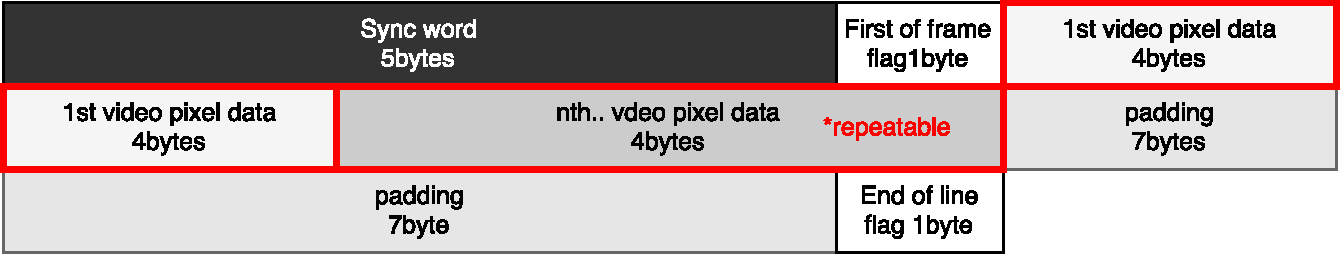
\includegraphics[bb=0 0 643 122,width=15.5cm]{img/fpga-video-packet.pdf}
  \end{center}
  \caption{UDPデータの構造}
  \label{fig:fpga-video-packet}
\end{figure}

UDPデータの映像データより前のヘッダー区間は6byteとなっている。
これは、FPGA内部でEthernetパケットを構築していく際に、データの先頭6byteが丁度64bitの区切り目となるためであり、FPGAで処理する祭に効率が良い。
UDPのパケットはFIFOにデータがある間生成され続けるため、IPパケット上の長さは00としている。映像データによってはジャンボフレームとなる場合もある。

各モジュールで映像データがどのように扱われるかを波形イメージとして、図~\ref{fig:fpga-first-pixel-waveform}に示す。

HDMI 1.4/2.0 Receiver Subsystemから出力されるデータは、v\_axi4s\_vid2fifo.vによって、1クロック遅れてFIFOに書き込まれる。
FIFOはある程度のバッファリングが行われるため、一定クロック経過後にemptyが立ち下がり、データが読み取れる状態となる。
v\_axi4s\_fifo2eth.vによって、emptyの立ち下がりの1クロック遅れで、Ethernet、IP、UDPヘッダーの生成を行う。ヘッダーの生成中にも映像データがFIFOにたまり続ける。
ヘッダーの生成がおわる1クロック前にrd\_enを立ち上げ、FIFOのデータを読み取る。UDPデータとして映像データを書き込み、almost\_emptyの立ち下がりでrd\_enを立ち下げる。
% 10 Gigabit Ethernet Subsystem

\begin{figure}[htbp]
  \begin{center}
    % \fbox{
    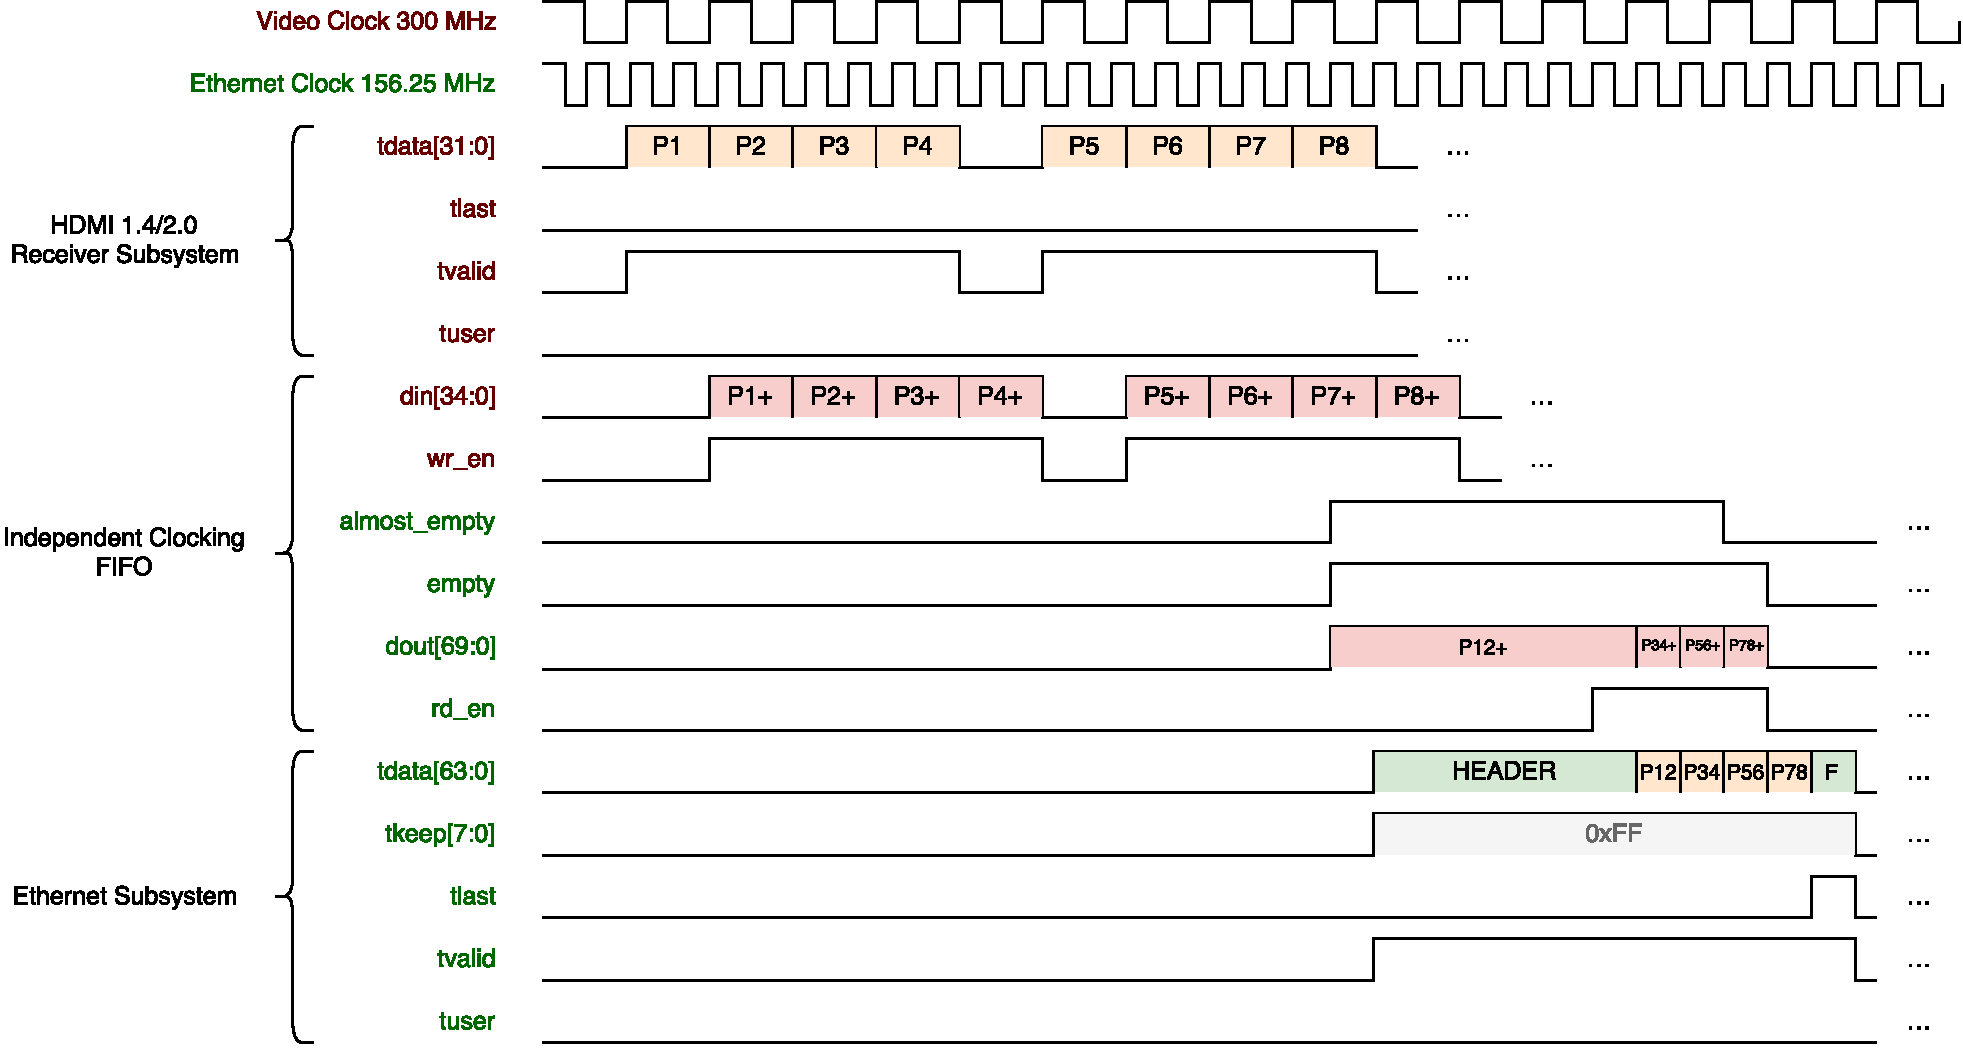
\includegraphics[bb=0 0 1118 502,width=22.5cm,angle=270]{img/fpga-first-pixel-waveform.pdf}
    % }
  \end{center}
  \caption{2つのクロックによるモジュール間でのデータ伝送の波形イメージ}
  \label{fig:fpga-first-pixel-waveform}
\end{figure}

% 図~\ref{fig:fpga-ila-fifo-to-eth}、
図~\ref{fig:fpga-ila-hdmi}では、本実装を稼働させたときのILA(Integrated Logic Analyzer)とよばれる、FPGAの内部信号をモニターするためのツールを使った際に、HDMIの入力と出力を検証した様子である。
前述の通り、almost\_emptyの立ち下がりを合図に、パケットを生成してから映像データを書き込むまでに一定のクロックが経過するため、FIFOへの書き込みがバッファリングされる。
hdmi\_rx\_tvalidが頻繁に立ち上がりと立ち下がりを繰り返しているのに対し、hdmi\_tx\_tvalidはある程度まとまった周期で立ち上がりをしている様子が確認できる。

% \begin{figure}[htbp]
%   \begin{center}
%     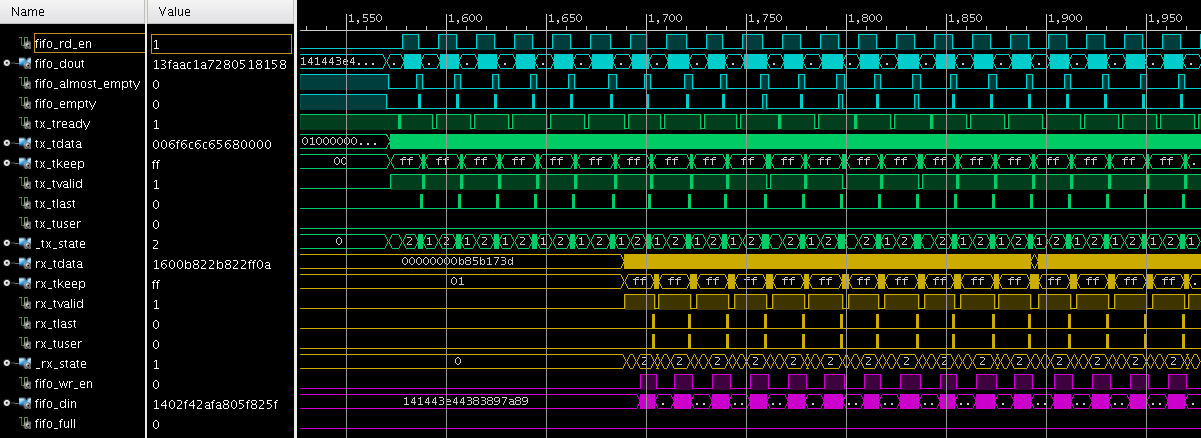
\includegraphics[bb=0 0 1201 438,width=15.5cm]{img/fpga-ila-fifo-to-eth.png}
%   \end{center}
%   \caption{ILAによるIP伝送時のFIFOとEthernet Subsystemのデータのダンプ}
%   \label{fig:fpga-ila-fifo-to-eth}
% \end{figure}

\begin{figure}[htbp]
  \begin{center}
    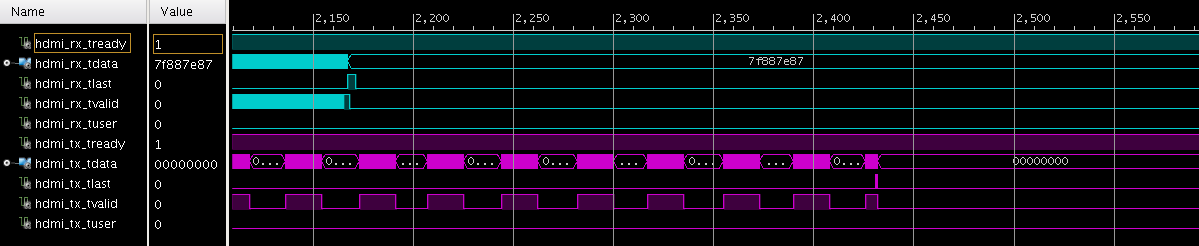
\includegraphics[bb=0 0 1199 246,width=22.5cm,angle=270]{img/fpga-ila-hdmi.png}
  \end{center}
  \caption{ILAによるIP伝送時のHDMI入出力のデータのダンプ}
  \label{fig:fpga-ila-hdmi}
\end{figure}

% \begin{figure}[htbp]
%     \begin{center}
%         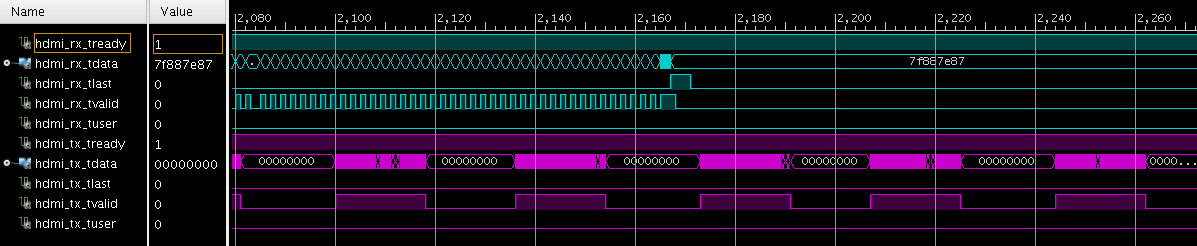
\includegraphics[bb=0 0 1197 246,width=15.5cm]{img/fpga-ila-hdmi-x2.png}
%     \end{center}
%     \caption{図~\ref{fig:fpga-ila-hdmi}を拡大した}
%     \label{fig:fpga-ila-hdmi-x2}
% \end{figure}

\begin{table}[htbp]
  \caption{論理合成後のリソース使用状況}
  \label{tb:fpga-post-implementation-utilization}
  \begin{center}
  \begin{tabular}{l|r|r|r}
    \hline
    リソース  & 使用    & 全体    & 使用率   \\\hline\hline
    LUT      &  48474 & 203800 & 23.79\% \\\hline
    LUTRAM   &   4696 &  64000 &  7.34\% \\\hline
    FF       &  55768 & 407600 & 13.68\% \\\hline
    BRAM     & 310.50 &    445 & 69.78\% \\\hline
    DSP      &     23 &    840 &  2.74\% \\\hline
    IO       &     40 &    500 &  8.00\% \\\hline
    GT       &      4 &     16 & 25.00\% \\\hline
    BUFG     &     20 &     32 & 62.50\% \\\hline
    MMCM     &      3 &     10 & 30.00\% \\\hline
    PLL      &      1 &     10 & 10.00\% \\\hline
  \end{tabular}\end{center}
\end{table}

\chapter{評価}
\label{chap:evaluation}
\section{評価手法}
\section{計測}
\subsection{トラフィック}
\subsection{遅延}
\subsection{重量}
\section{考察}

\chapter{結論}
\label{chap:conclusion}
\section{本研究のまとめ}
\section{今後の課題と展望}


\begin{acknowledgment}

本研究を進めるにあたり、ご指導いただきました慶應義塾大学 環境情報学部教授 村井純博士、同学部教授 中村修博士、同学部准教授 Rodney D. Van Meter III 博士、同学部准教授 植原啓介博士、同学部准教授 中澤仁博士、SFC 研究所 上席所員 (訪問) 斉藤賢爾博士に感謝致します。

研究について日頃からご指導頂きました松谷健史博士、空閑洋平博士、理工学研究科開放環境科学専攻 後期博士課程 徳差雄太氏に感謝致します。
研究室に所属したばかりの頃から本研究に至るまで、特定の分野にこだわらない広い視点で何年生の時であっても妥協のない姿勢で向かい合い、絶えず多くのご指導をいただきました。
本研究を卒業論文としてまとめることができたのも両氏のおかげです。重ねて感謝申し上げます。

本研究の評価に必要な伝送装置の助言、機材を運搬していただいた一般社団法人 Mozilla Japan 工藤紀篤博士に感謝いたします。
評価に必要な伝送装置を借用させていただいた慶應義塾大学デジタルメディア・コンテンツ統合研究センターの皆様に感謝いたします。
長期の間、開発、実験用に4Kカメラなどの機器を借用させていただいた慶應義塾大学湘南藤沢メディアセンターマルチメディアサービスの皆様に感謝いたします。
実証実験を行ったORF2015では、実行委員会の皆様、ネットワーク環境を整備していただいたITCの皆様、ORF NOCの皆様、映像制作をしていただいた音像工房の皆様に感謝いたします。
本研究のハードウェア実装にあたっての資金援助をいただきました、山岸プロジェクトの山岸広太郎氏、関係者の皆様に感謝いたします。

研究室を通じた生活の中で多くの示唆を与えてくれた阿部涼介氏、沖幸太朗氏、木下舜氏、黒米祐馬氏、鈴木恒平氏、\CID{8705}橋佑允氏、原雅彦氏、細田航星氏、およびArch研究グループの皆様に感謝します。
また、徳田・村井・楠本・中村・高汐・バンミーター・植原・三次・中澤・武田 合同研究プロジェクトの皆様に感謝致します。

最後に、私の研究を支えてくれた両親をはじめとする親族、多くの友人・知人に感謝し、謝辞と致します。

\end{acknowledgment}
  % 謝辞。要独自コマンド、include先参照のこと
\include{section/91_bibliography}  % 参考文献。要独自コマンド、include先参照のこと

\appendix
\chapter{ORF2015での100Gbps回線を使用した映像伝送と遠隔スイッチングの実証実験}
\label{chap:orf2015}

\section{実験の構成}
\begin{figure}[htbp]
    \begin{center}
        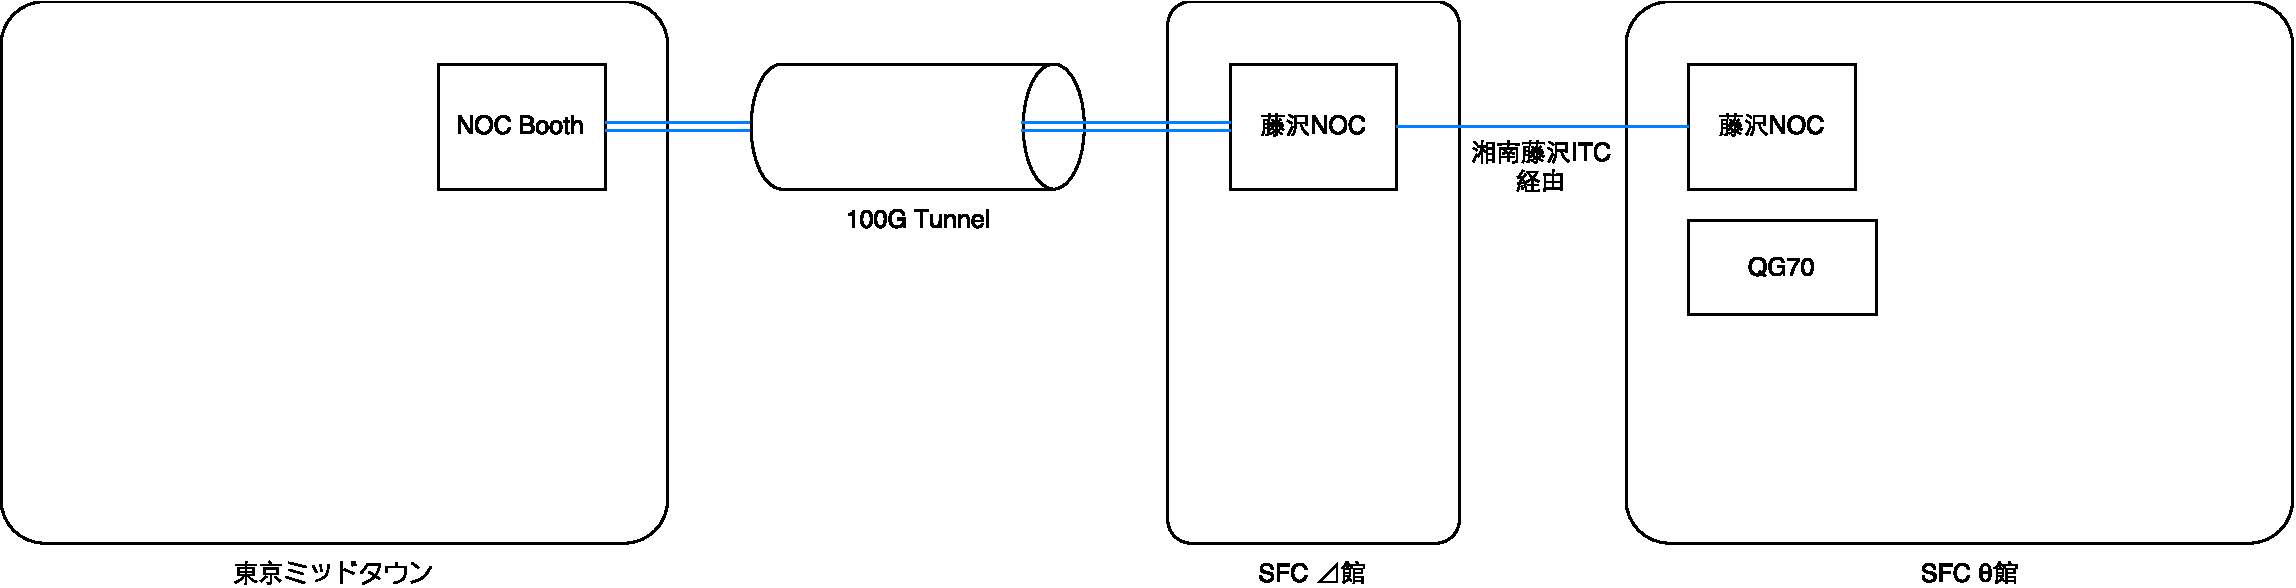
\includegraphics[bb=0 0 1101 282,width=15.5cm]{img/orf2015-flow.pdf}
    \end{center}
    \caption{ORF2015での実験の構成}
    \label{fig:orf2015-flow}
\end{figure}

\begin{figure}[htbp]
    \begin{center}
        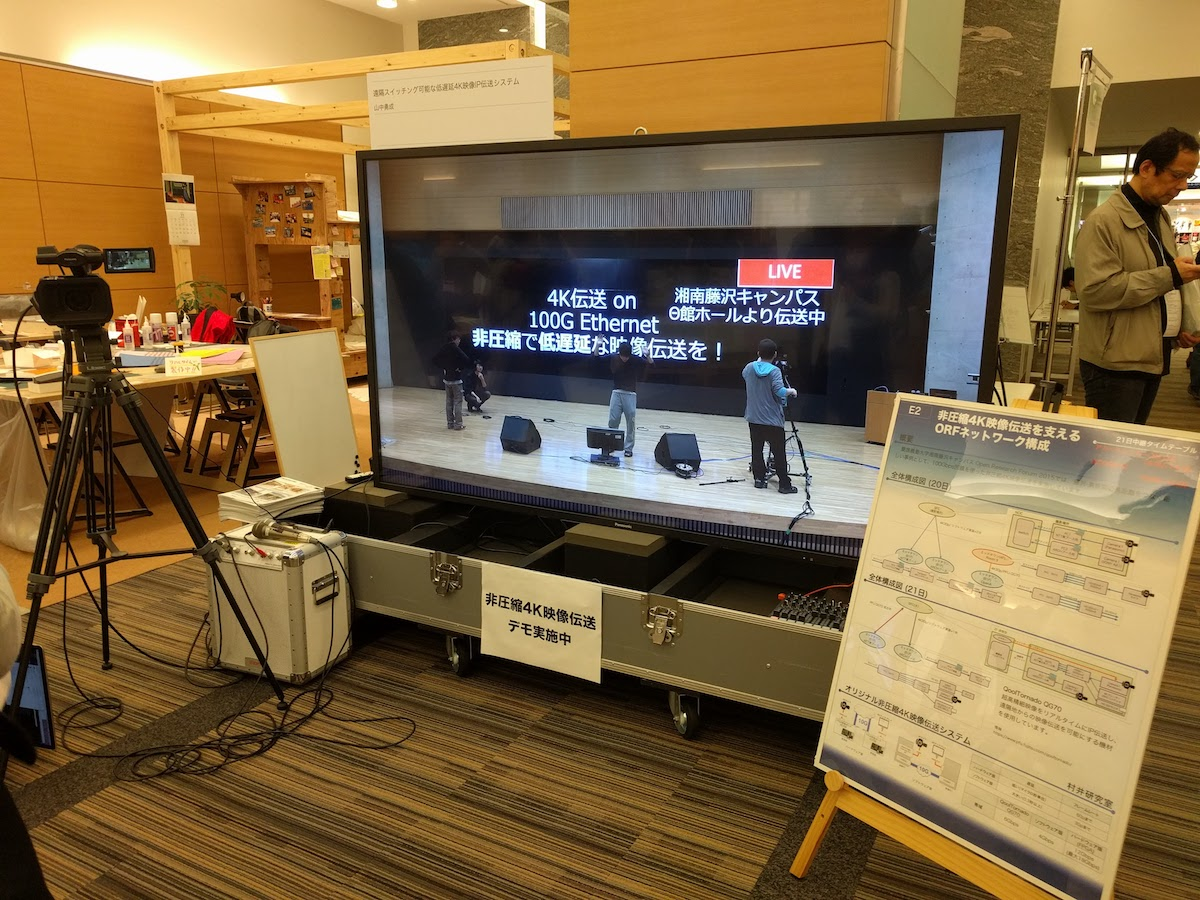
\includegraphics[bb=0 0 1200 900,width=15.5cm]{img/orf2015-IMG_20151121_132910.jpg}
    \end{center}
    \caption{ORF2015での実証実験の様子}
    \label{fig:orf2015-IMG_20151121_132910}
\end{figure}


\section{遠隔スイッチング}

\chapter{ORF2016での実証実験}
\label{chap:orf2016}
\section{実験の構成}
    % 付録

\end{document}
